% =====================================================================
% EOLLM: Earth-Observation + Language-Model Dataset — Technical Report
% =====================================================================
% Compile:
%     pdflatex main.tex   (twice, for ToC/refs)
% All figures are vector PDFs; example QA panels are PNG photographs.
% =====================================================================
\documentclass[11pt,a4paper]{article}

% ---------- packages ----------
\usepackage[utf8]{inputenc}
\usepackage[T1]{fontenc}
\usepackage{lmodern}
\usepackage[margin=2.2cm]{geometry}
\usepackage{graphicx}
\usepackage{xcolor}
\usepackage{booktabs}
\usepackage{tabularx}
\usepackage{array}
\usepackage{caption}
\usepackage{subcaption}
\usepackage{hyperref}
\usepackage{enumitem}
\usepackage{tcolorbox}
\usepackage{microtype}
\usepackage{titlesec}
\usepackage{multicol}
\usepackage{multirow}
\usepackage{float}
\usepackage{listings}

\definecolor{eollmblue}{HTML}{1F77B4}
\definecolor{eollmorange}{HTML}{FF7F0E}
\definecolor{eollmgreen}{HTML}{2CA02C}
\definecolor{boxbg}{HTML}{F5F8FC}
\definecolor{boxrule}{HTML}{1F77B4}

\hypersetup{
  colorlinks=true,
  linkcolor=eollmblue,
  citecolor=eollmblue,
  urlcolor=eollmblue,
  pdftitle={EOLLM Dataset Technical Report},
  pdfauthor={EOLLM Team},
}

\captionsetup{font=small, labelfont={bf,color=eollmblue}, skip=4pt}

\titleformat{\section}{\Large\bfseries\color{eollmblue}}{\thesection.}{0.6em}{}
\titleformat{\subsection}{\large\bfseries}{\thesubsection.}{0.5em}{}
\titlespacing*{\section}{0pt}{1.4em}{0.6em}

\newtcolorbox{infobox}[1][]{
  colback=boxbg, colframe=boxrule, boxrule=0.6pt,
  arc=2pt, left=8pt, right=8pt, top=4pt, bottom=4pt,
  fonttitle=\bfseries, title=#1,
}

\lstset{
  basicstyle=\ttfamily\small,
  breaklines=true,
  showstringspaces=false,
  frame=single,
  framerule=0.4pt,
  rulecolor=\color{gray!40},
  backgroundcolor=\color{boxbg},
  xleftmargin=2pt, xrightmargin=2pt,
  aboveskip=6pt, belowskip=6pt,
}

% ---------- title ----------
\title{\vspace{-1.2cm}\textcolor{eollmblue}{\textbf{EOLLM}}\\
       \large A Multi-City Visual Question Answering Dataset for\\
       Urban Understanding and Cross-View Geolocalisation}
\author{EOLLM Project --- Technical Report}
\date{Generated \today}

\begin{document}
\maketitle
\thispagestyle{empty}
\vspace{-1em}

\begin{abstract}
\noindent
EOLLM is a multiple-choice Visual Question Answering (VQA) dataset that pairs
high-resolution satellite imagery with Google Street View panoramas
across \textbf{40 cities in 32 countries}, and asks Vision-Language Models
(VLMs) a fixed catalogue of \textbf{14 question types} that probe urban
understanding and cross-view geolocalisation. The released corpus contains
\textbf{39{,}155 question records} grounded in \textbf{4{,}168 unique
locations}; ground-truth labels are derived deterministically from
OpenStreetMap tags --- no manual annotation, no third-party geocoder. The
dataset ships with three split strategies (per-city, seen/unseen cities, and
a held-out benchmark) so that researchers can measure both
in-distribution location understanding and geographic generalisation under
the same task taxonomy. This report documents the data sources, the
generation pipeline, the task taxonomy, the statistical composition, known
limitations, and the file layout of the compressed release
(\texttt{EODATA\_compressed\_final}, $\sim$7\,GB).
\end{abstract}

\begin{infobox}[At a glance]
\begin{tabularx}{\linewidth}{@{}lXlX@{}}
\textbf{Cities}            & 40   & \textbf{Question records (release)} & 39{,}155 \\
\textbf{Countries}         & 32   & \textbf{Unique sample locations}    & 4{,}168 \\
\textbf{Question types}    & 14   & \textbf{Split strategies}           & 3 \\
\textbf{Images per loc.}   & 1 sat + 4 SV & \textbf{Compressed size}    & $\sim$7\,GB \\
\end{tabularx}
\end{infobox}

\tableofcontents
\newpage

% =====================================================================
\section{Introduction}
% =====================================================================

\subsection{Motivation}
Modern Vision-Language Models are evaluated mostly on web-scraped images
that mix objects, charts and natural scenes. Two abilities important for
real-world deployment are largely absent from these benchmarks:

\begin{enumerate}[itemsep=2pt]
  \item \textbf{Urban understanding} --- judging land use, building stock,
        transit access, or pedestrian environment from a single
        location, where the model must integrate signals across modalities.
  \item \textbf{Cross-view geolocalisation} --- reasoning about whether two
        viewpoints (overhead and ground-level) refer to the same place,
        or pointing out which compass direction a photo was taken from.
\end{enumerate}

\noindent EOLLM was built to fill that gap with a single, internally
consistent corpus: every question links one ground-truth location to
exactly one satellite tile and four Street View images, and the
correct option is derived from OpenStreetMap rather than human labelling.

\subsection{Design principles}
\begin{itemize}[itemsep=2pt]
  \item \textbf{Deterministic ground truth.} All answers come from
        OSM tags and geometric calculations. Re-running the pipeline
        on the same OSM snapshot yields the same answers, with no
        annotator drift.
  \item \textbf{Multi-modal by default.} The default visual is a
        composite of satellite and Street View; the question schema
        records exactly which visual to assemble.
  \item \textbf{Reproducible question generation.} Option order is
        shuffled with a per-question RNG seeded from
        \texttt{sample\_id} + \texttt{topic}, so the dataset is
        bit-exact regenerable.
  \item \textbf{Two splits, one taxonomy.} The same question types are
        evaluated under both \emph{per-city} (held-out locations within
        seen cities) and \emph{seen/unseen cities} (held-out entire
        cities) regimes, plus a disjoint benchmark.
\end{itemize}

% =====================================================================
\section{Dataset Construction}
% =====================================================================
The pipeline runs in seven stages, each a self-contained Python script
under \texttt{src/}. The orchestrator (\texttt{run\_pipeline.py})
threads sample dictionaries through every stage and writes the
final JSONL.

\begin{figure}[H]
  \centering
  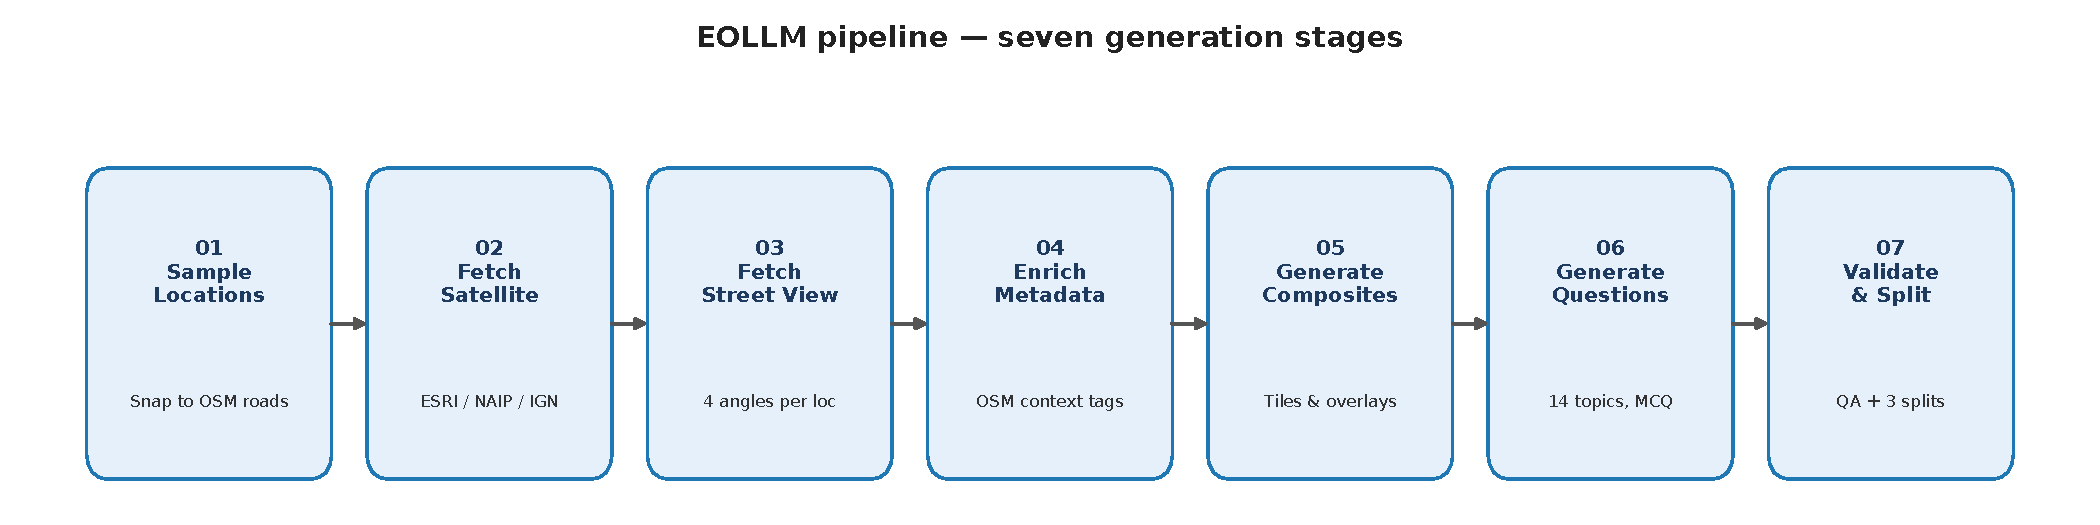
\includegraphics[width=\linewidth]{figures/fig13_pipeline.pdf}
  \caption{Seven-stage data generation pipeline. Every stage reads and
  enriches the same list of sample dictionaries.}
  \label{fig:pipeline}
\end{figure}

\subsection{Location sampling (Step 01)}
Sample points are generated inside each city's bounding box and
snapped to the nearest OSM road segment whose tag matches
\texttt{primary | secondary | tertiary | residential | trunk}.
Motorways are excluded because Street View along them is largely
useless for urban tasks and biases the \texttt{road\_type}
distribution. The target is \texttt{SAMPLES\_PER\_CITY = 120}; the actual unique-location
yield per city across the release (\texttt{splits\_per\_city} +
\texttt{benchmark}) ranges from \textbf{50} (Nairobi) to \textbf{120}
(Budapest) with a median of \textbf{110} (Fig.~\ref{fig:locs}).
Restricted to \texttt{splits\_per\_city} alone, the median drops to
\textbf{99} since benchmark-only locations are excluded.

\subsection{Satellite imagery (Step 02)}
Each location gets one $512\times512$ satellite tile. The provider is
auto-selected by coordinates:
\begin{itemize}[itemsep=0pt]
  \item \textbf{NAIP} (USDA, $\sim$0.6\,m/pixel) --- United States.
  \item \textbf{IGN} ($\sim$0.2\,m/pixel) --- France.
  \item \textbf{ESRI World Imagery} ($\sim$0.3--0.5\,m/pixel in cities) --- global default.
  \item \textbf{Sentinel-2} (10\,m/pixel) --- fallback only when the
        primary source returns a tile smaller than 5\,kB.
\end{itemize}
In the released 39{,}155-record corpus ESRI covers \textbf{35{,}609}
questions (91\%), NAIP \textbf{2{,}294}, and IGN \textbf{1{,}252}; no
Sentinel-2 fallback was triggered in the final release.

\subsection{Street View (Step 03)}
Four panoramas are pulled per location, each rotated to a road-aligned
heading: \texttt{along\_fwd}, \texttt{along\_bwd}, \texttt{cross\_left},
\texttt{cross\_right}. Locations with no SV coverage (e.g., the
indoor-only Canary Wharf area of London) are dropped at this stage.
A simple RGB-channel-spread heuristic ($>40$) rejects tunnel imagery.

\subsection{OSM enrichment (Step 04)}
Each sample is annotated with OSM context inside a small buffer
(typically 100--300\,m): building footprints and \texttt{building:levels},
amenity nodes, leisure/park polygons, water bodies, transit stops,
and junction types from way intersections. These tags are the source
of the deterministic answers for the urban-understanding tasks.

\subsection{Composite images (Step 05)}
For task-specific visuals (red-dot marker on the satellite, arrows
pointing in each MCQ option's direction, $2\times2$ Street View grids,
or $4\times4$ mega-grids of four candidate locations), composites are
either pre-rendered to disk (during pipeline construction) or
re-generated on the fly at training time from raw images via
\texttt{composite\_utils.py}. The compressed release relies on the
on-the-fly path.

\subsection{Question generation (Step 06)}
Templates produce MCQ options from the OSM-derived ground truth and
sample plausible distractors from the same category space.
Per-question RNG (seeded from \texttt{sample\_id} + topic) shuffles
option order so that the correct letter is stable across re-runs
but distributed across letters in the corpus.

\subsection{Validation \& splitting (Step 07)}
Records are filtered for image availability and OSM completeness, then
divided into three disjoint splits:
\textbf{(a)} per-city train/val (random within each city),
\textbf{(b)} seen/unseen train/val (8 cities held out entirely), and
\textbf{(c)} a benchmark drawn from a disjoint mixture of seen and
unseen cities. The benchmark is shipped in two parallel files
(\texttt{public}, no answers; \texttt{with\_answers}, gold-labelled).

% =====================================================================
\section{Task Taxonomy}
% =====================================================================

The 14 question types split into two families: \emph{urban
understanding} (the answer follows from one location's OSM context)
and \emph{cross-view geolocalisation} (the answer follows from the
relationship between modalities or the camera geometry).

\begin{figure}[H]
  \centering
  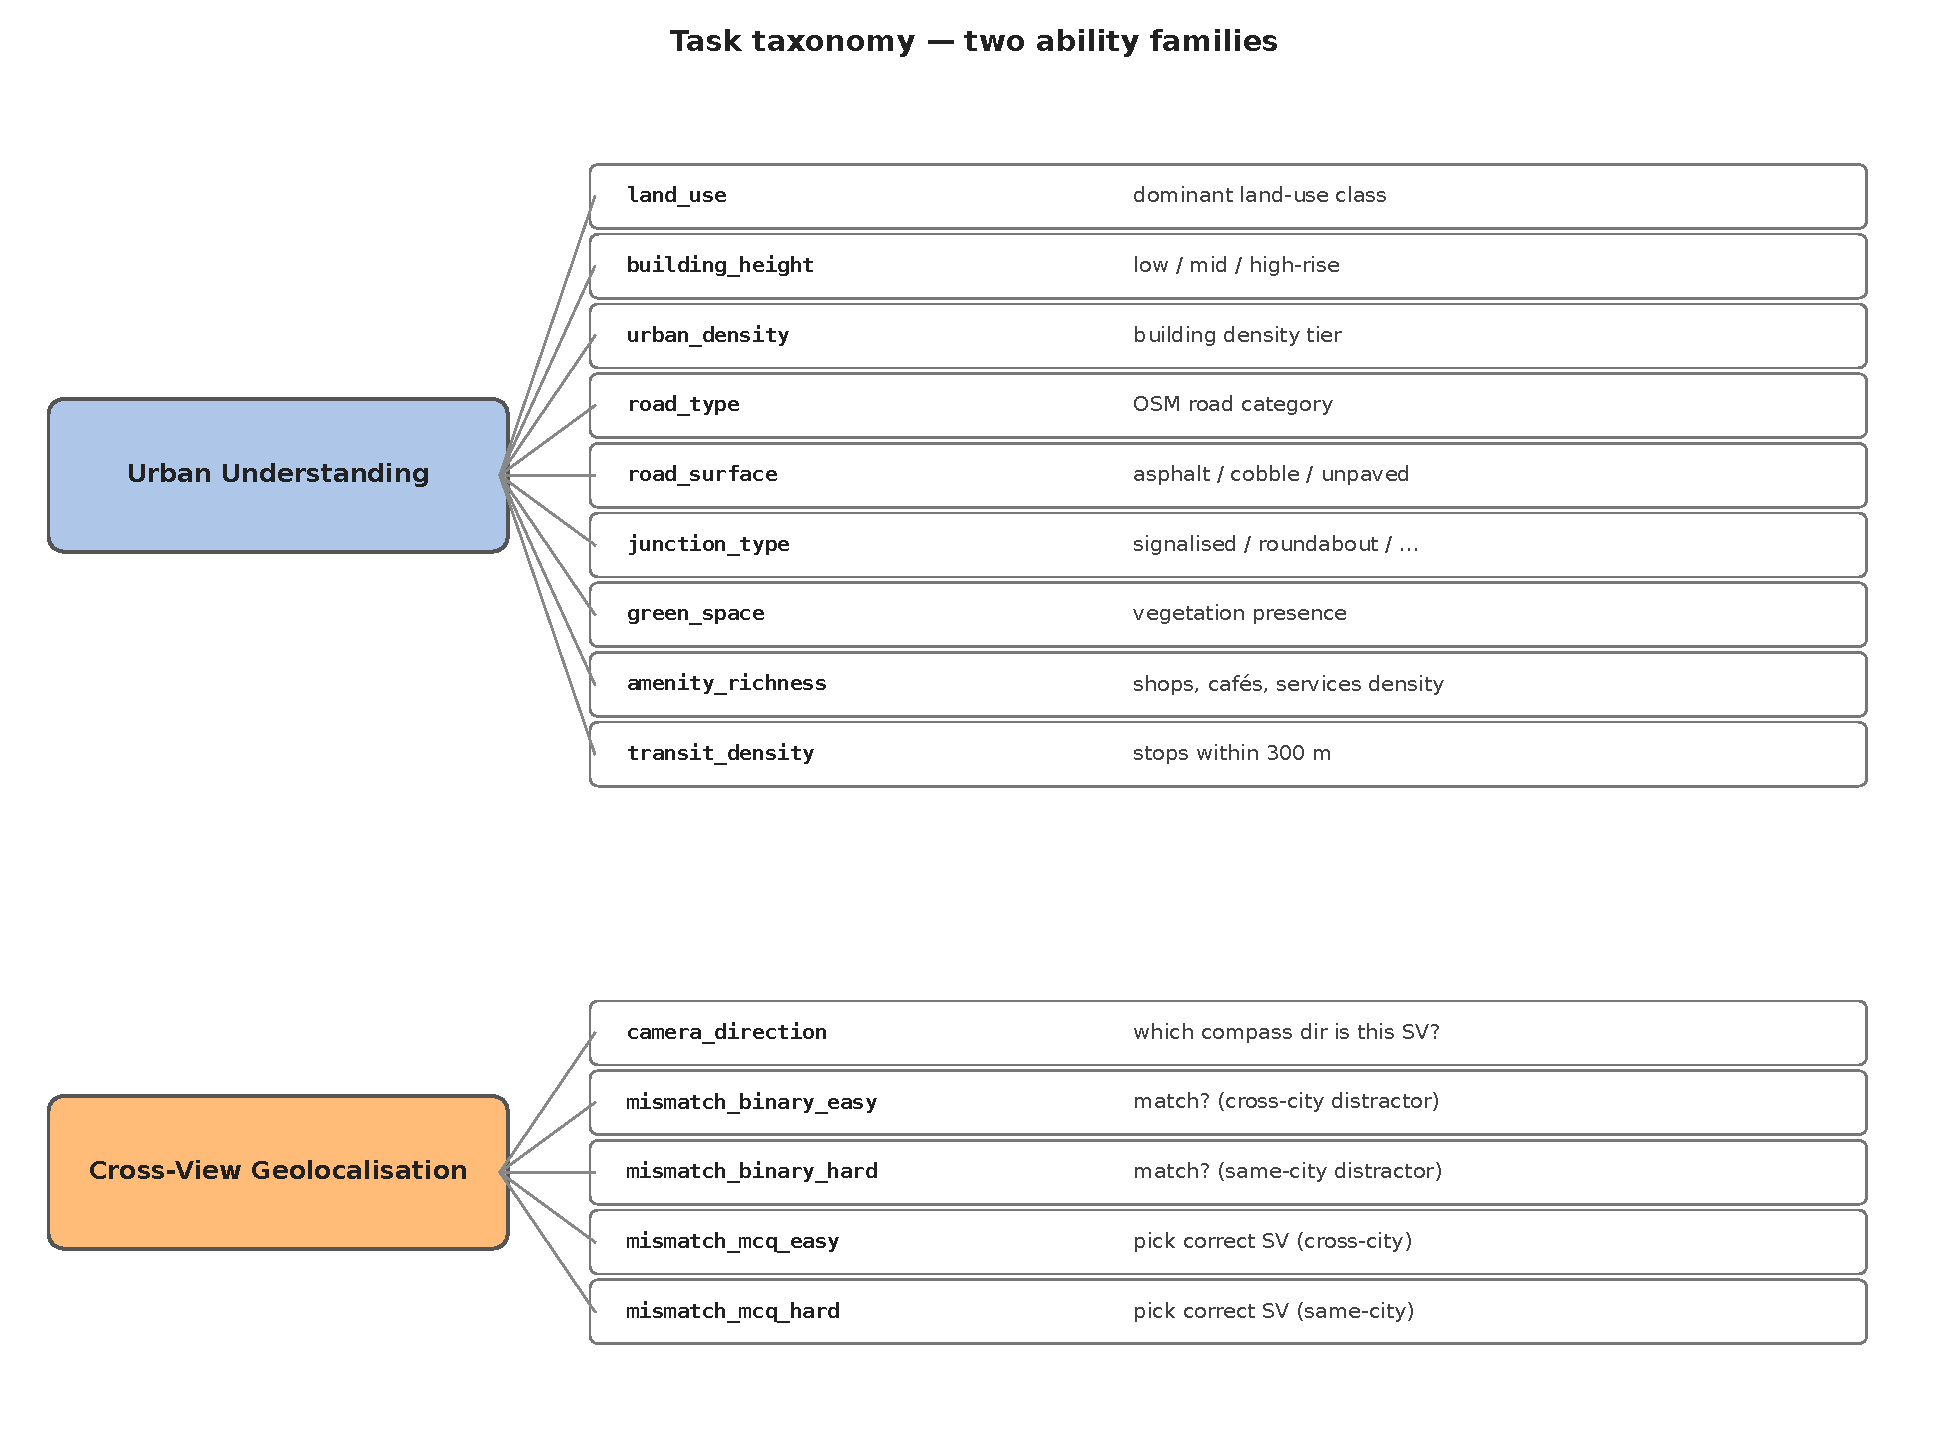
\includegraphics[width=0.92\linewidth]{figures/fig14_task_taxonomy.pdf}
  \caption{The 14 question types organised by the ability they
  probe. Mismatch types are split into easy (cross-city distractor)
  and hard (same-city distractor).}
  \label{fig:taxonomy}
\end{figure}

\subsection{What each task measures}

\renewcommand{\arraystretch}{1.2}
\begin{tabularx}{\linewidth}{@{}>{\ttfamily\small}l p{4.6cm} X@{}}
\toprule
\textnormal{\textbf{Topic}} & \textbf{Visual} & \textbf{Ability tested} \\
\midrule
land\_use         & satellite + red dot              & Reading dominant urban morphology from overhead. \\
building\_height  & satellite + red dot              & Estimating built-form scale; reasoning from texture and shadow. \\
urban\_density    & satellite + red dot              & Counting / density estimation in a fixed radius. \\
road\_type        & satellite + red dot              & Inferring road class from carriageway width, surroundings. \\
road\_surface     & satellite + red dot              & Fine-grained material recognition; cobblestone vs.\ asphalt. \\
junction\_type    & satellite + red dot              & Recognising intersection topology (roundabout, signalised, etc.). \\
green\_space      & satellite + red dot              & Vegetation segmentation and proximity reasoning. \\
amenity\_richness & satellite + red dot              & Inferring service availability from urban texture. \\
transit\_density  & satellite + red dot              & Counting public-transit infrastructure. \\
camera\_direction & satellite + arrow per option + 1 SV & Cross-view orientation: align a ground view with an overhead arrow. \\
mismatch\_binary\_easy & 4-angle SV grid             & Same-location verification with cross-city distractor. \\
mismatch\_binary\_hard & 4-angle SV grid             & Same-location verification with same-city distractor (much harder). \\
mismatch\_mcq\_easy    & 4$\times$4 mega-grid (4 candidates $\times$ 4 angles) & Pick-the-match among visually-similar street views (cross-city). \\
mismatch\_mcq\_hard    & 4$\times$4 mega-grid (4 candidates $\times$ 4 angles) & Pick-the-match within the same city (intra-city distractors). \\
\bottomrule
\end{tabularx}

\subsection{Mismatch tasks --- the geolocalisation core}
The mismatch family is the most discriminative subset of the dataset.
\emph{Easy} variants draw the distractor from another city, where
ambient cues (vegetation, sky, signage language, vehicle types) often
leak the answer. \emph{Hard} variants draw the distractor from the
same city, defeating those shortcuts and isolating the geometric
match between satellite layout and ground-level structure.

% =====================================================================
\section{Dataset Statistics}
% =====================================================================

The released corpus contains \textbf{39{,}155 question records}
(per-city train + per-city val + benchmark). The
\texttt{splits\_seen\_unseen} folder re-uses the same locations under
a different train/val partition; aggregating both strategies yields
\textbf{48{,}332 unique question identifiers}.

\subsection{Splits}

\begin{table}[H]
  \centering\small
  \begin{tabular}{lrrr}
  \toprule
  \textbf{Split set} & \textbf{Train} & \textbf{Validation} & \textbf{Benchmark} \\
  \midrule
  per\_city          & 26{,}931 & 6{,}984 & --- \\
  seen\_unseen       & 26{,}963 & 8{,}831 & --- \\
  benchmark          & ---      & ---     & 5{,}240 (public) / 5{,}240 (w/ answers) \\
  \bottomrule
  \end{tabular}
  \caption{Record counts per split. \texttt{seen\_unseen} validation
  holds out 8 entire cities; \texttt{per\_city} validation holds out
  random locations inside every city.}
  \label{tab:splits}
\end{table}

\begin{figure}[H]
  \centering
  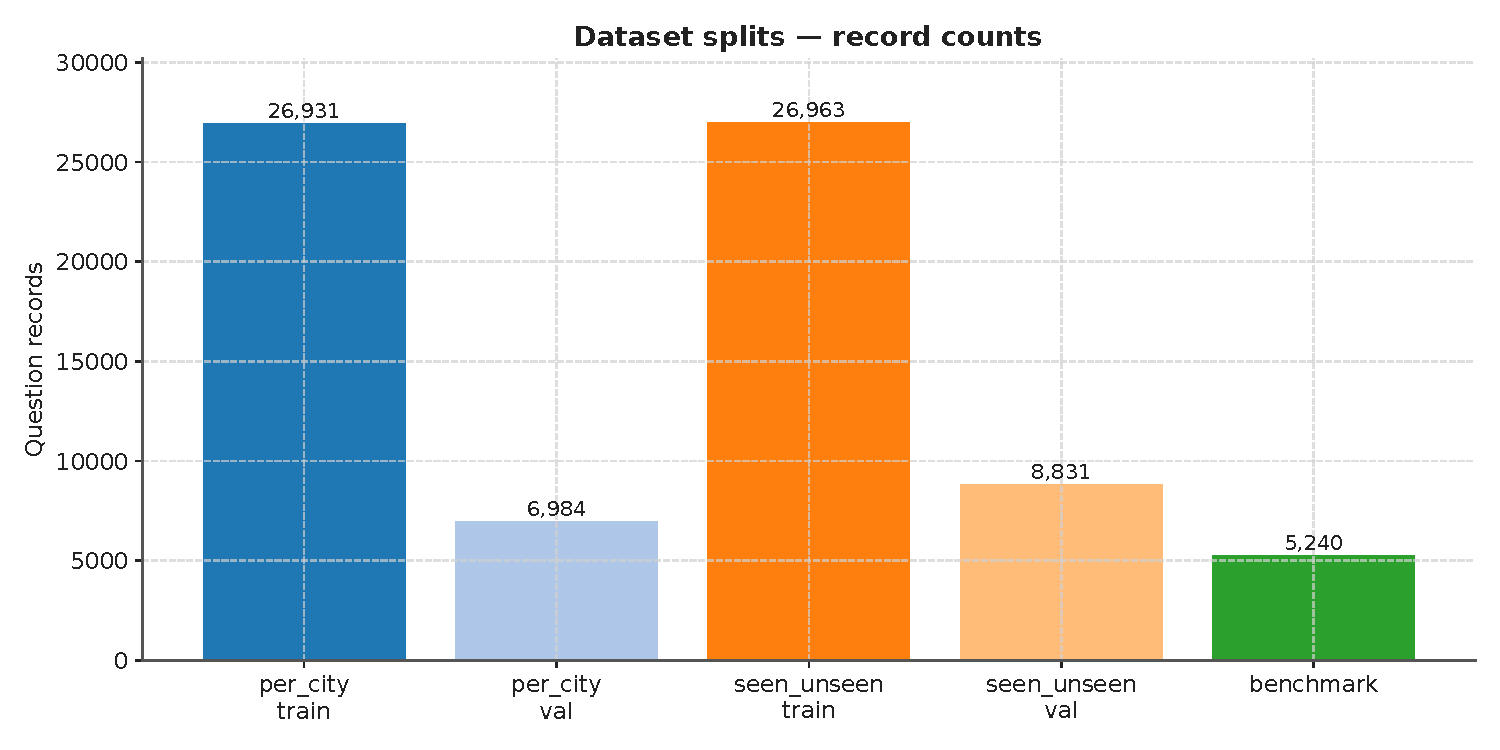
\includegraphics[width=0.85\linewidth]{figures/fig05_splits.pdf}
  \caption{Record counts per split. The two split strategies share
  most underlying locations and questions; the benchmark is
  fully disjoint from both.}
  \label{fig:splits}
\end{figure}

\subsection{Question types}

\begin{figure}[H]
  \centering
  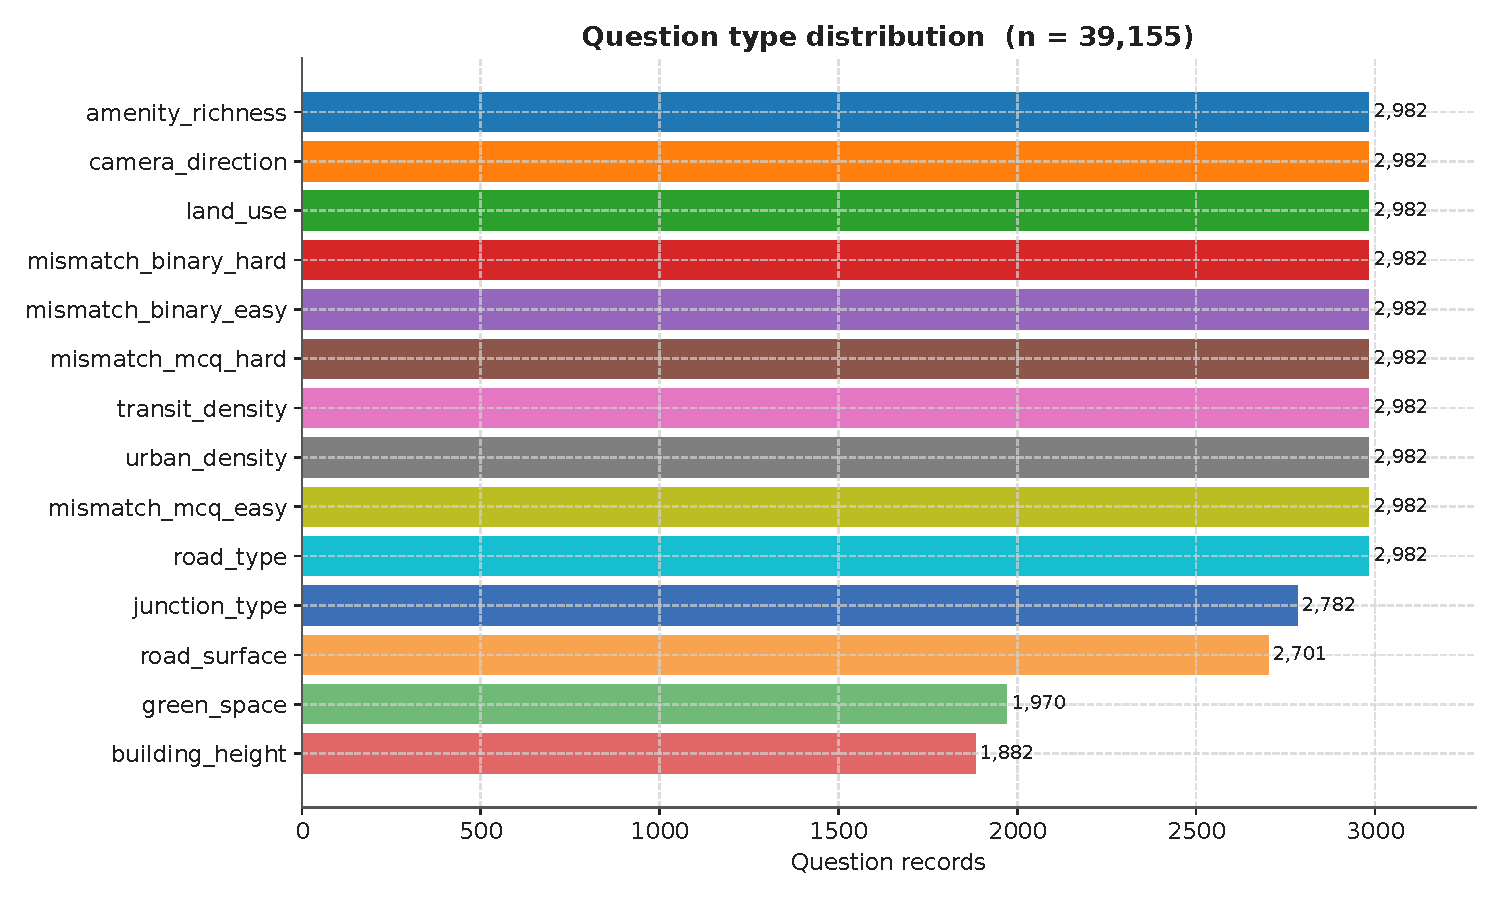
\includegraphics[width=\linewidth]{figures/fig01_topic_distribution.pdf}
  \caption{Distribution of question records across the 14 topics.
  The ten "balanced" topics each contribute roughly 2{,}982 records;
  \texttt{junction\_type}, \texttt{road\_surface}, \texttt{green\_space} and
  \texttt{building\_height} are smaller because they require OSM tags
  that are not present at every location.}
  \label{fig:topics}
\end{figure}

\begin{figure}[H]
  \centering
  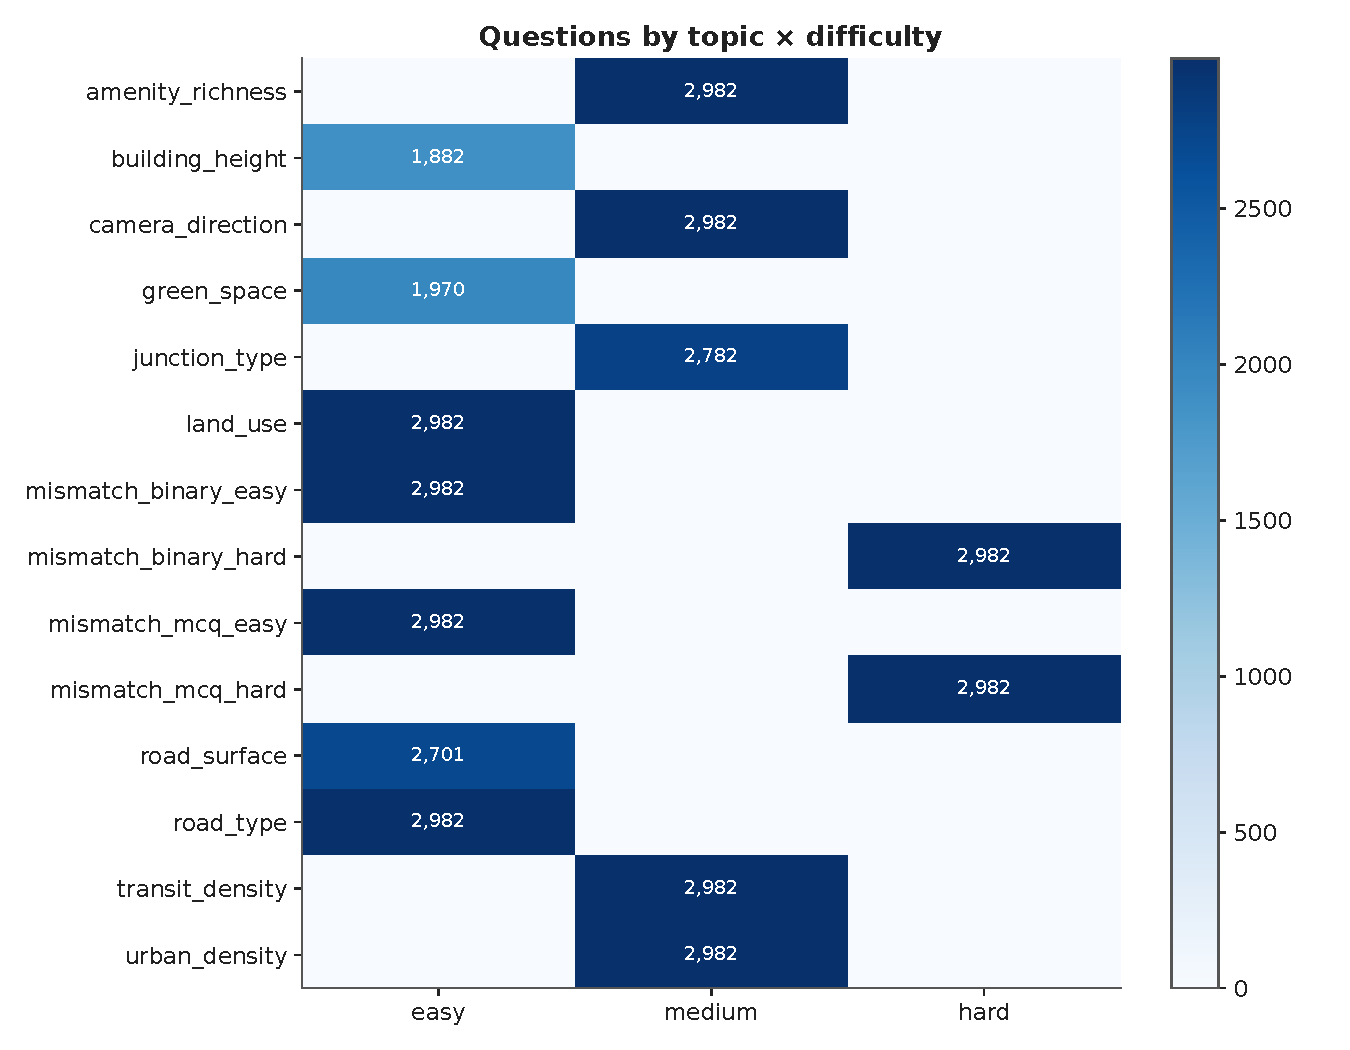
\includegraphics[width=0.95\linewidth]{figures/fig09_topic_vs_difficulty.pdf}
  \caption{Topic $\times$ difficulty matrix. \texttt{hard} entries are
  concentrated in the \texttt{mismatch\_*\_hard} topics, where the
  distractor is drawn from the same city as the target.}
  \label{fig:topicdiff}
\end{figure}

\subsection{Geographic coverage}

\begin{figure}[H]
  \centering
  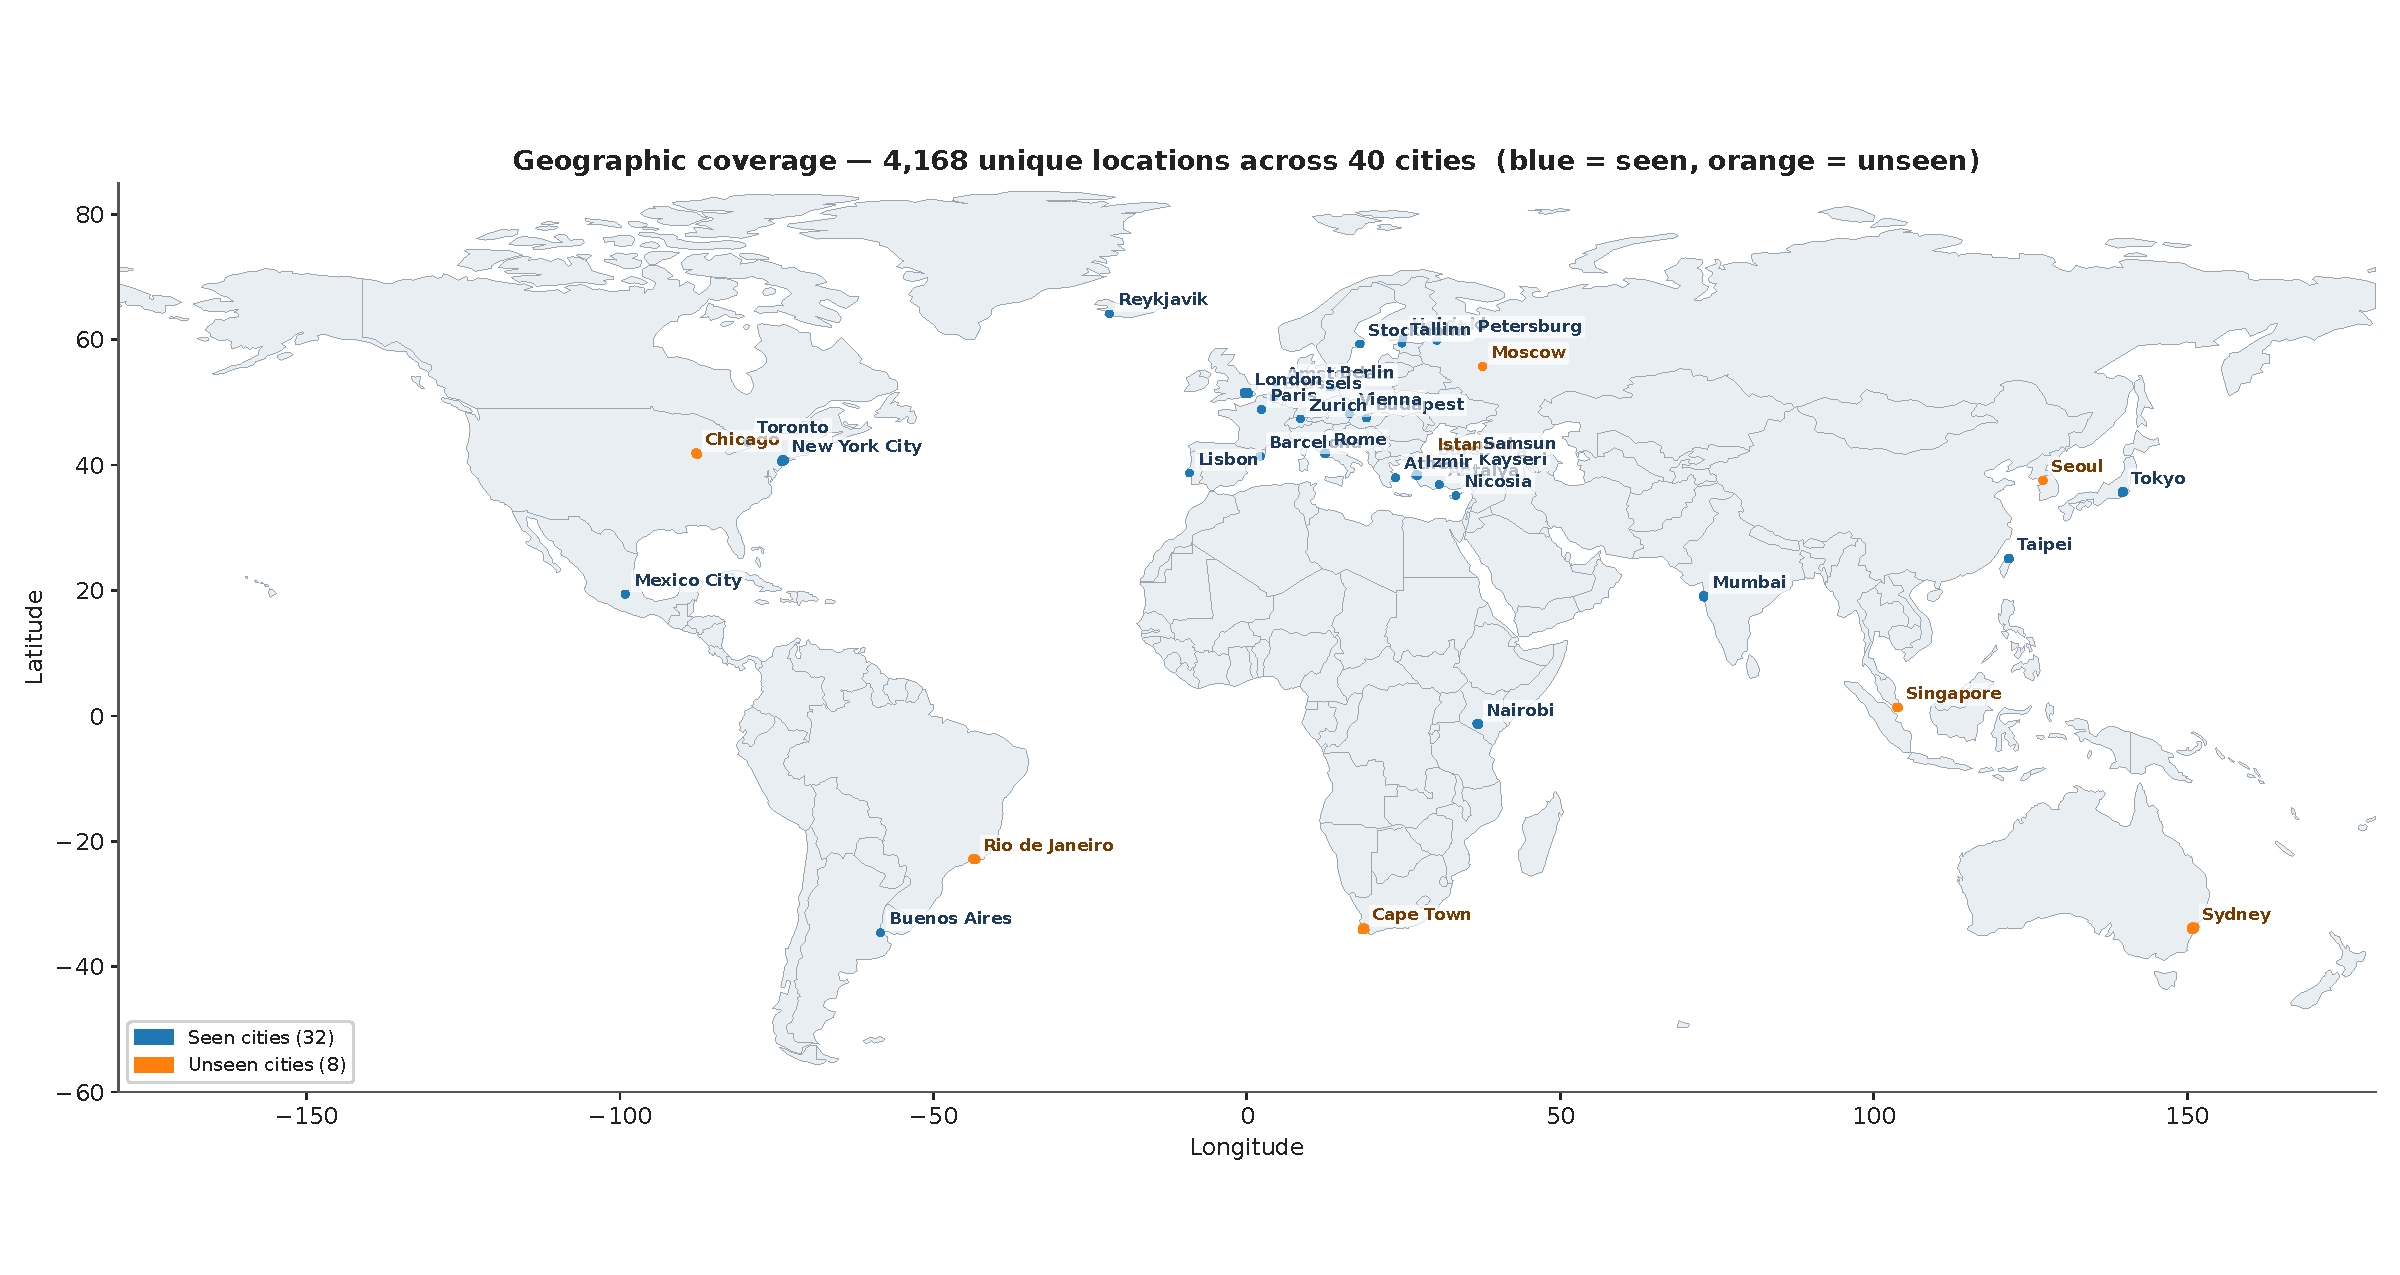
\includegraphics[width=\linewidth]{figures/fig11_geographic_scatter.pdf}
  \caption{Locations of the 4{,}168 unique samples on a world map.
  Blue = "seen" cities (32) used in
  \texttt{splits\_seen\_unseen} training; orange = "unseen" cities
  (8) held out for geographic-generalisation evaluation.}
  \label{fig:geo}
\end{figure}

\begin{figure}[H]
  \centering
  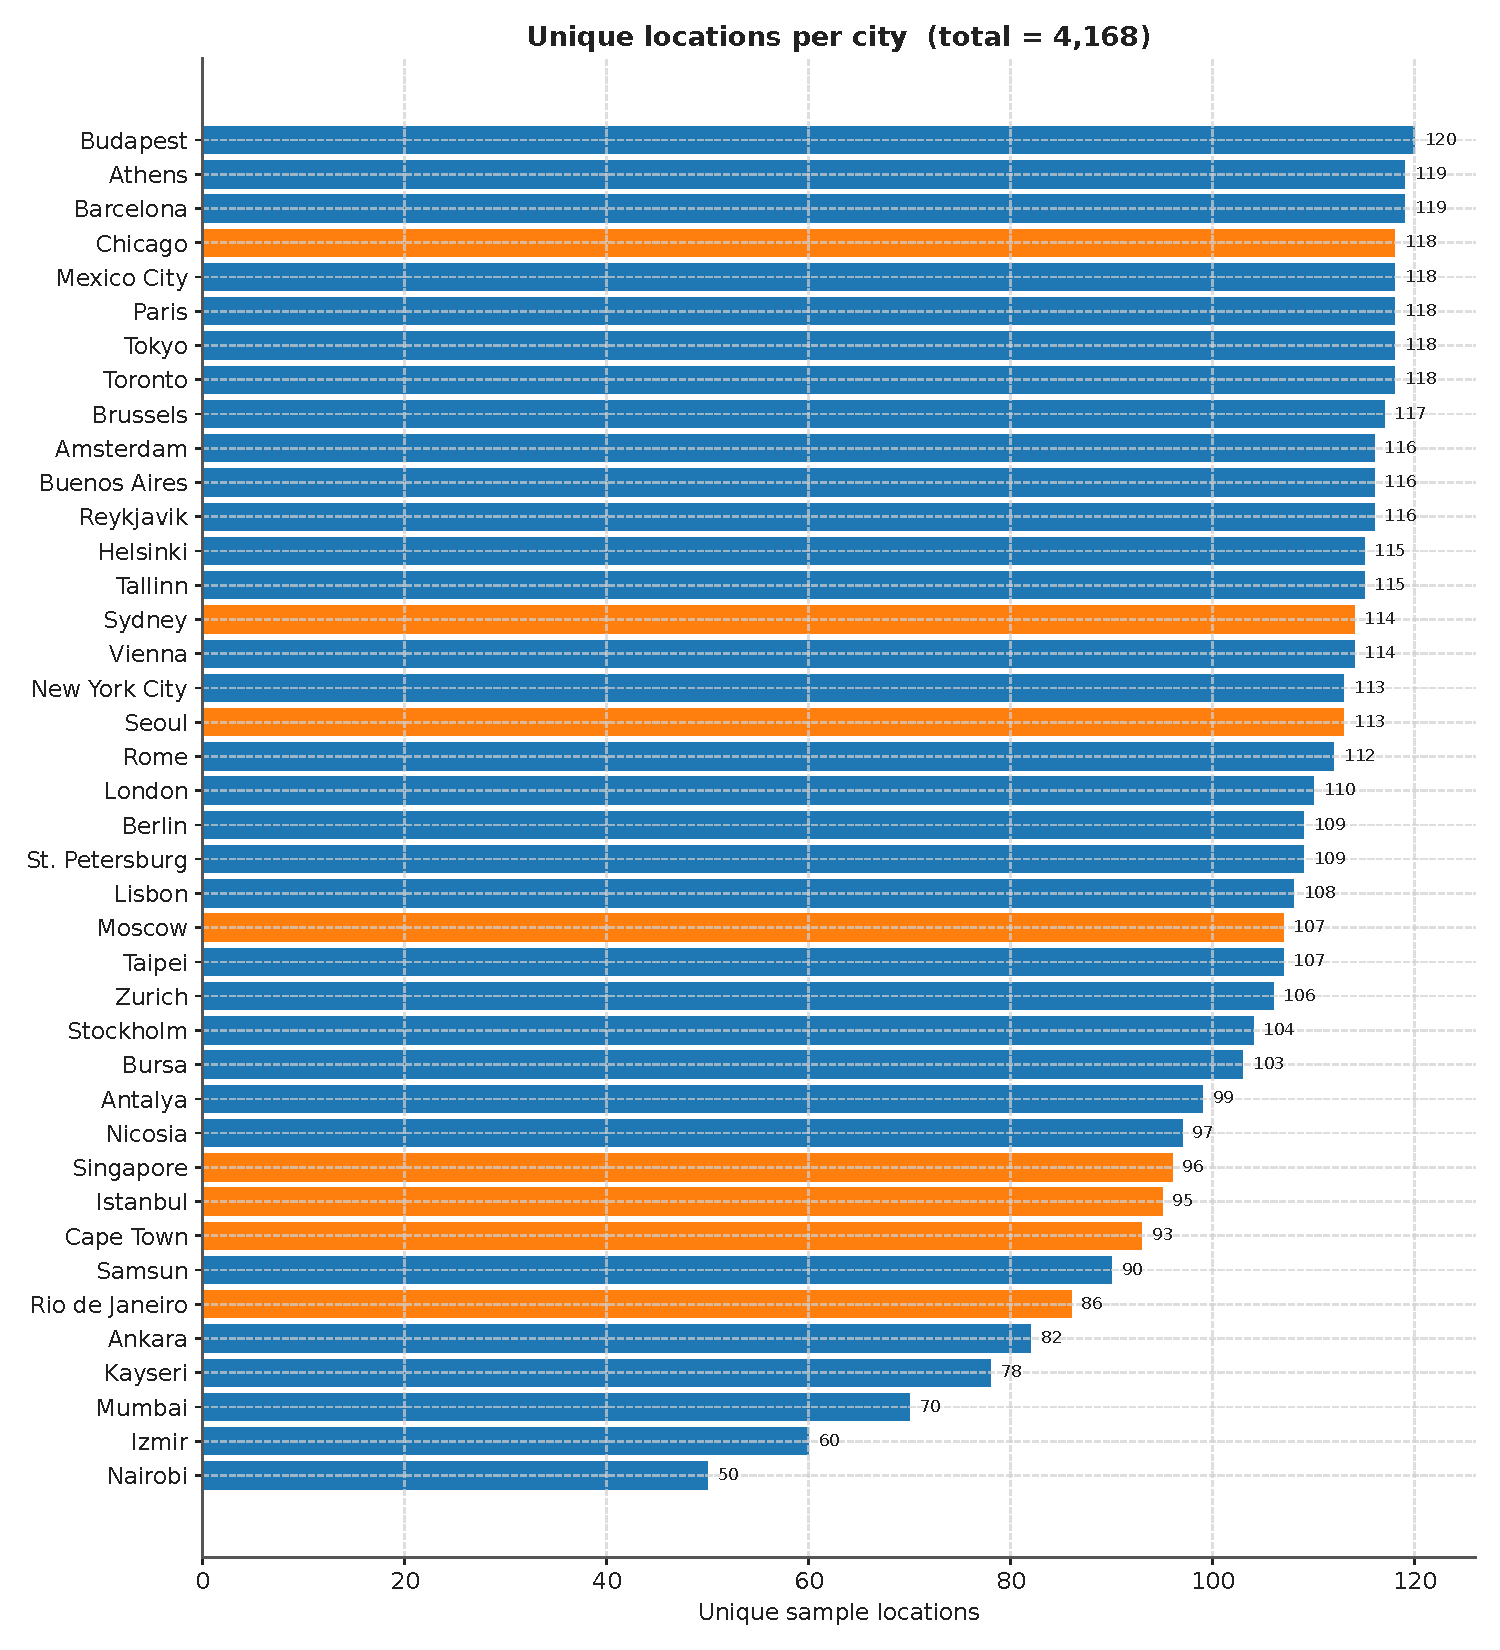
\includegraphics[width=0.92\linewidth]{figures/fig03_locations_per_city.pdf}
  \caption{Unique sample locations per city. The configured target is
  120 per city; the actual yield depends on road coverage,
  Street View availability, and OSM completeness.}
  \label{fig:locs}
\end{figure}

\begin{figure}[H]
  \centering
  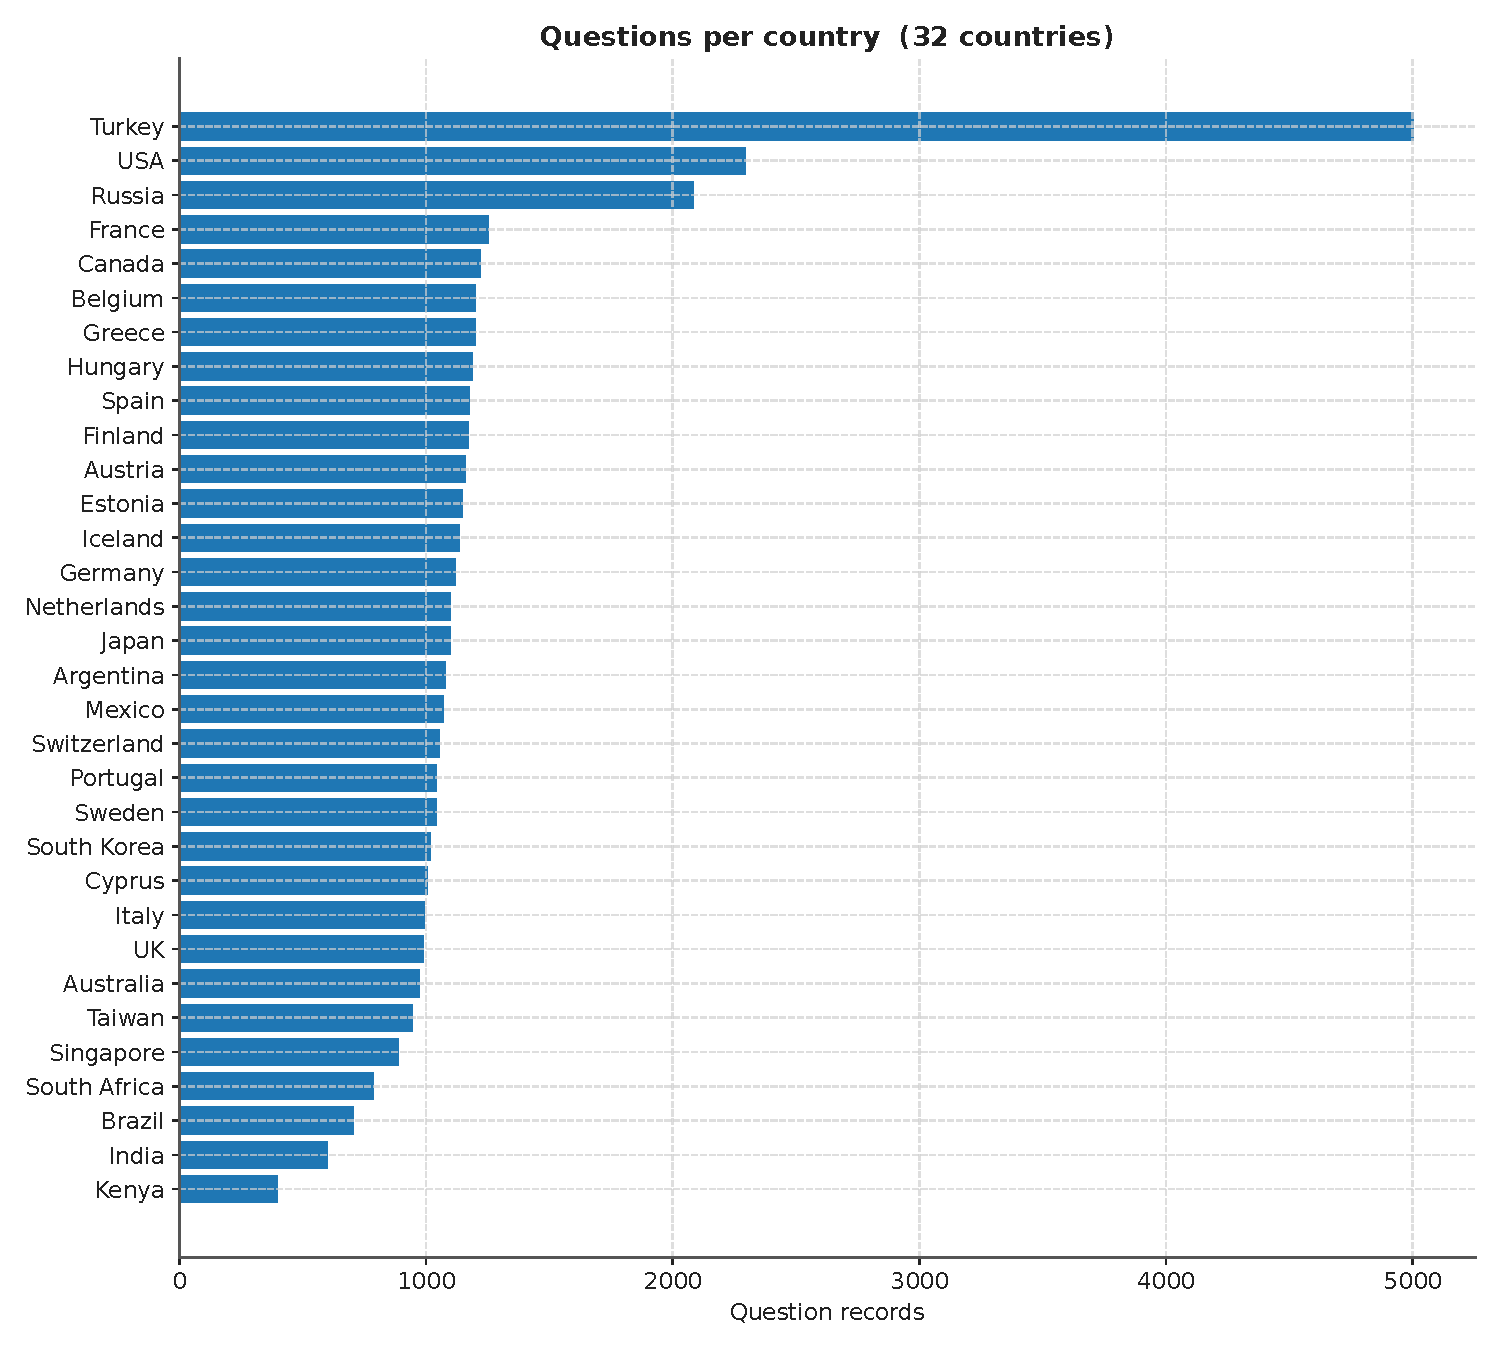
\includegraphics[width=0.92\linewidth]{figures/fig04_countries.pdf}
  \caption{Question records per country. The 40 cities span 32
  countries (after merging the spellings \emph{Turkey} and
  \emph{Turkiye} that appear in the raw JSONL).}
  \label{fig:countries}
\end{figure}

\subsection{Modality and content composition}

\begin{figure}[H]
  \centering
  \begin{subfigure}{0.49\linewidth}
    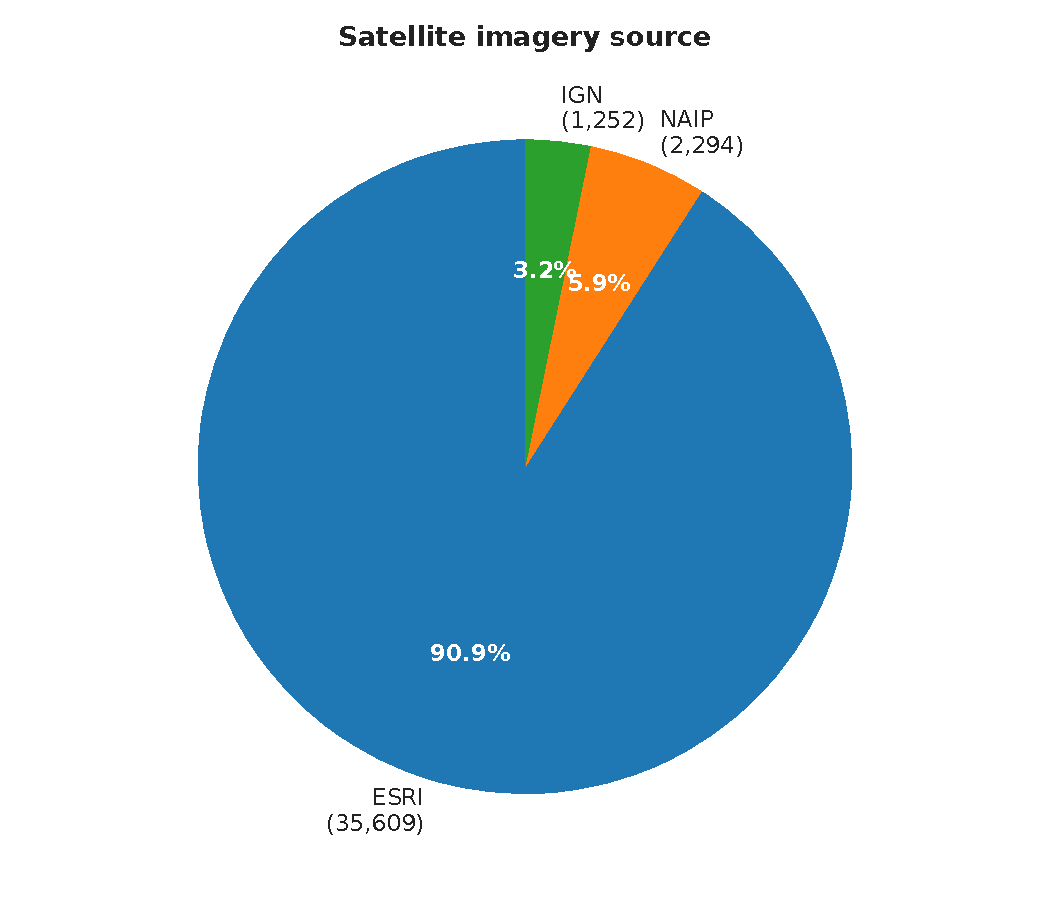
\includegraphics[width=\linewidth]{figures/fig08_sat_source.pdf}
    \caption{Satellite imagery provider.}
  \end{subfigure}
  \hfill
  \begin{subfigure}{0.49\linewidth}
    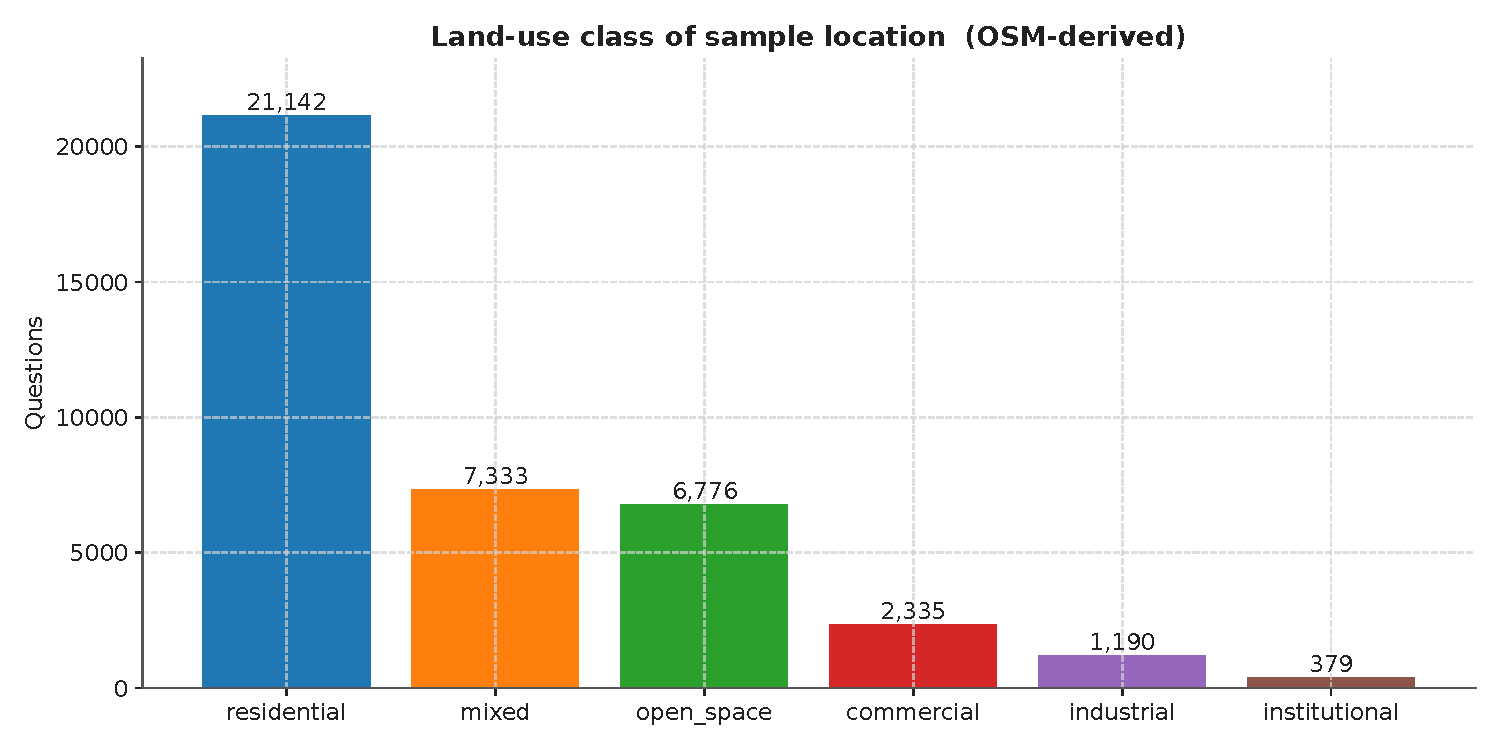
\includegraphics[width=\linewidth]{figures/fig07_land_use.pdf}
    \caption{Dominant land-use class.}
  \end{subfigure}
  \caption{Imagery sources and OSM-derived land-use mix.}
  \label{fig:sourcesland}
\end{figure}

\begin{figure}[H]
  \centering
  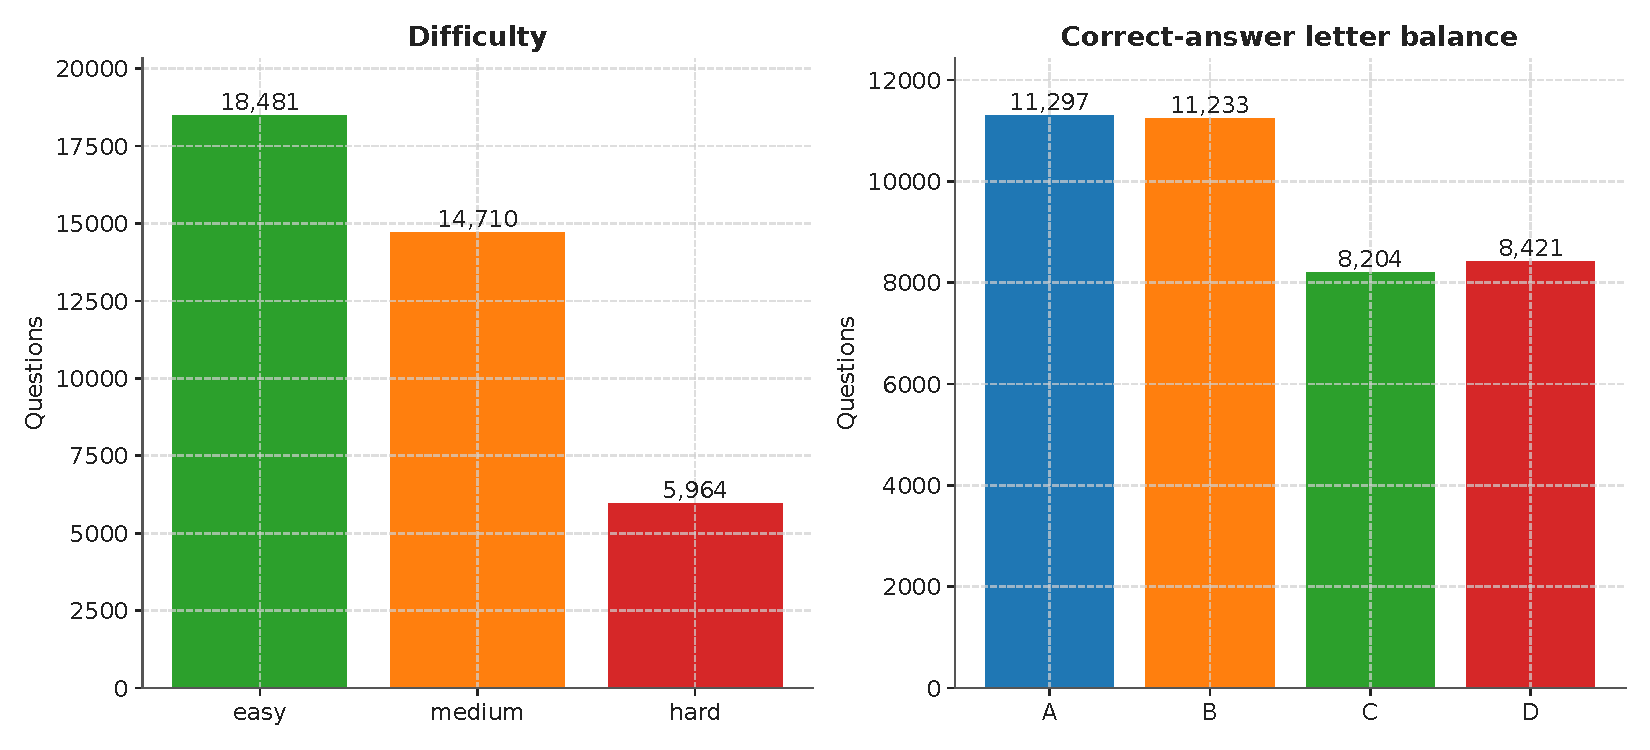
\includegraphics[width=\linewidth]{figures/fig06_difficulty_answer.pdf}
  \caption{Difficulty labels and correct-letter distribution.
  Letters A and B occur more often than C and D: this is a known
  artefact of the option-shuffling RNG and is documented in
  \S\ref{sec:limits}.}
  \label{fig:diffans}
\end{figure}

\begin{figure}[H]
  \centering
  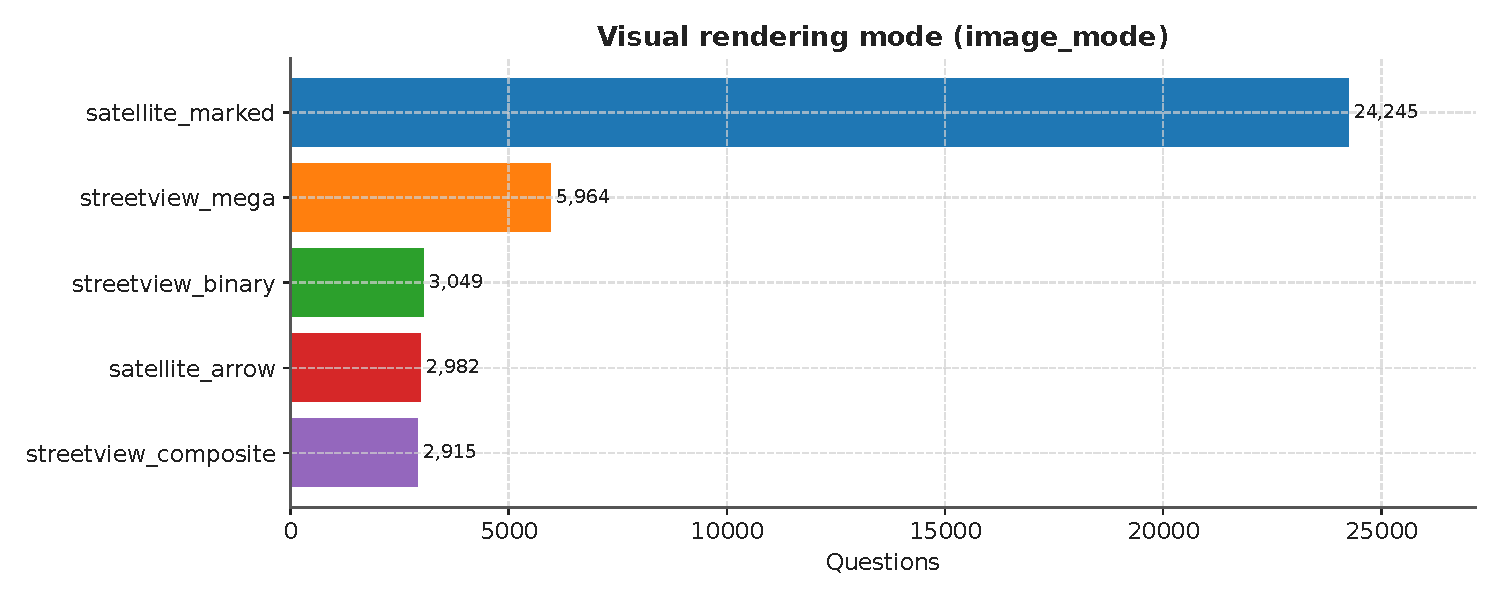
\includegraphics[width=0.92\linewidth]{figures/fig12_image_modes.pdf}
  \caption{The \texttt{image\_mode} field tells the dataloader which
  visual to assemble. \texttt{satellite\_marked} is the default for
  the nine urban-understanding topics; the remaining four modes
  handle camera-direction and mismatch tasks.}
  \label{fig:imagemodes}
\end{figure}

\begin{figure}[H]
  \centering
  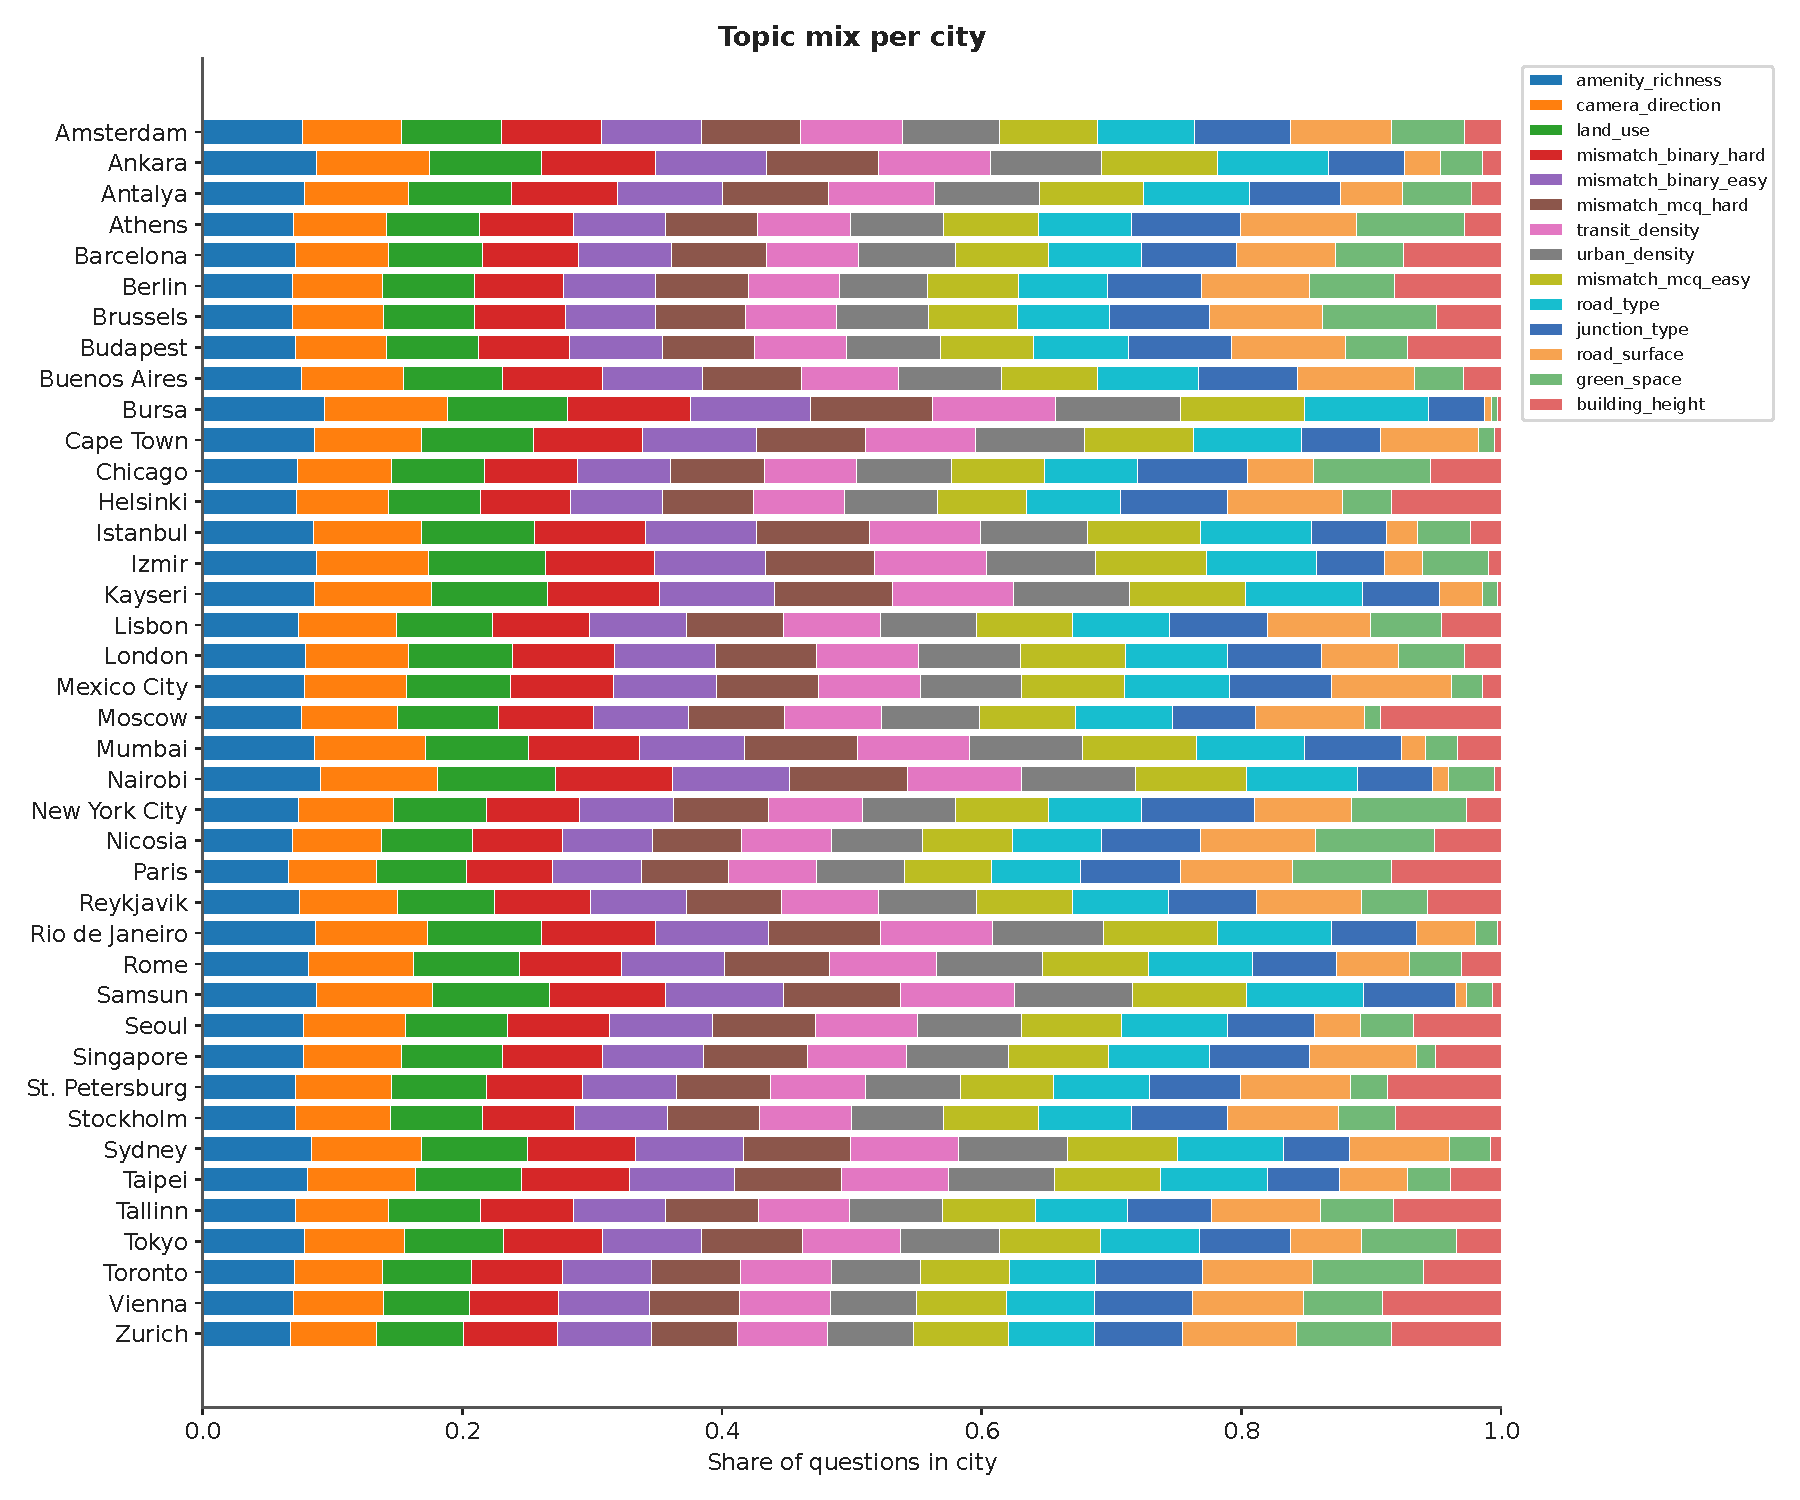
\includegraphics[width=\linewidth]{figures/fig10_topic_mix_per_city.pdf}
  \caption{Topic mix per city. The shape is nearly uniform across
  cities, with small deviations driven by OSM-tag sparsity (e.g.\
  \texttt{building:levels} is sparse in São Paulo and Singapore,
  reducing \texttt{building\_height} records there).}
  \label{fig:topicmix}
\end{figure}

% =====================================================================
\section{Example Questions}
\label{sec:examples}
% =====================================================================
Each panel below shows the actual rendered visual that the model
receives at evaluation time, together with the question, the four
options, and the gold answer.

\subsection{Urban-understanding examples}

\begin{figure}[H]
  \centering
  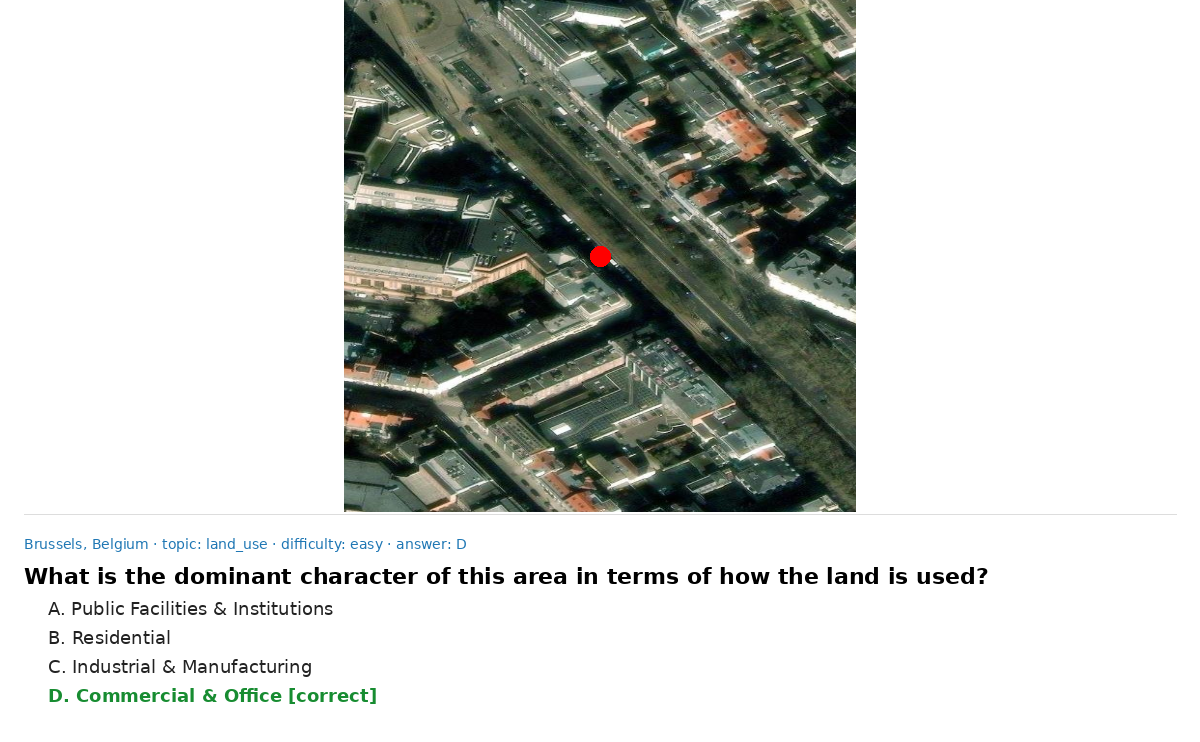
\includegraphics[width=0.9\linewidth]{examples/ex_land_use.png}
  \caption{\texttt{land\_use} --- dominant urban morphology from overhead.}
\end{figure}

\begin{figure}[H]
  \centering
  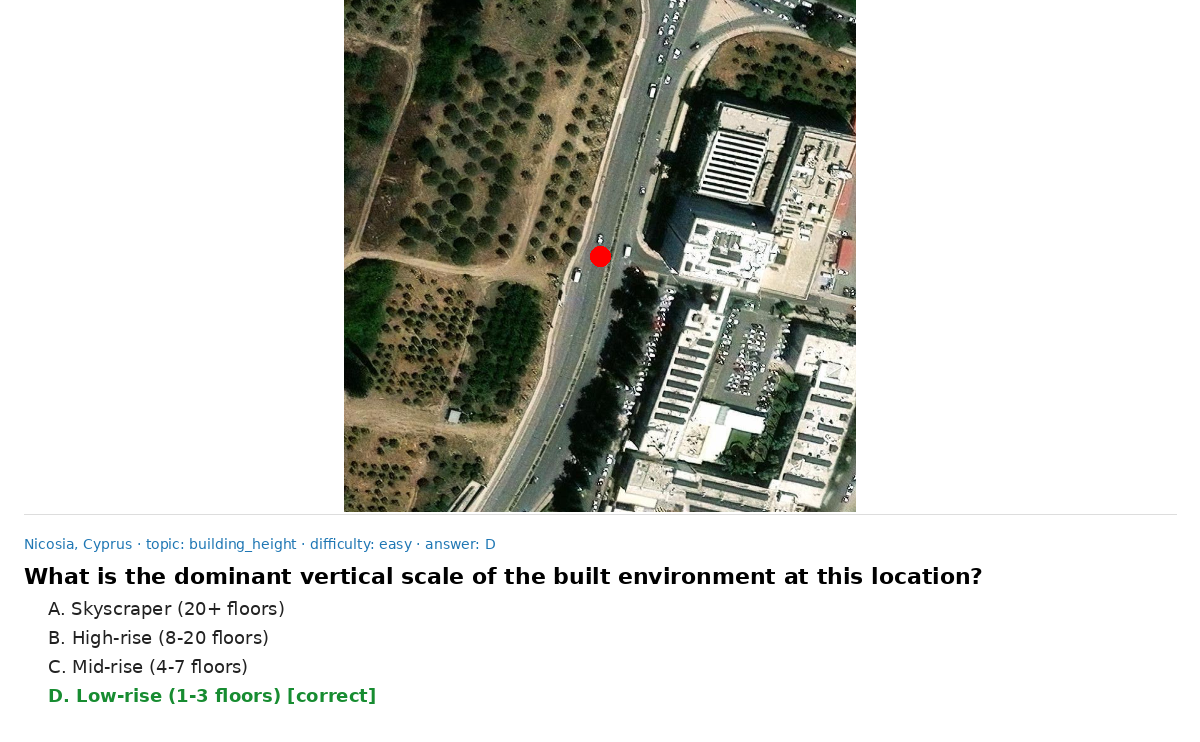
\includegraphics[width=0.9\linewidth]{examples/ex_building_height.png}
  \caption{\texttt{building\_height} --- low / mid / high-rise tier.}
\end{figure}

\begin{figure}[H]
  \centering
  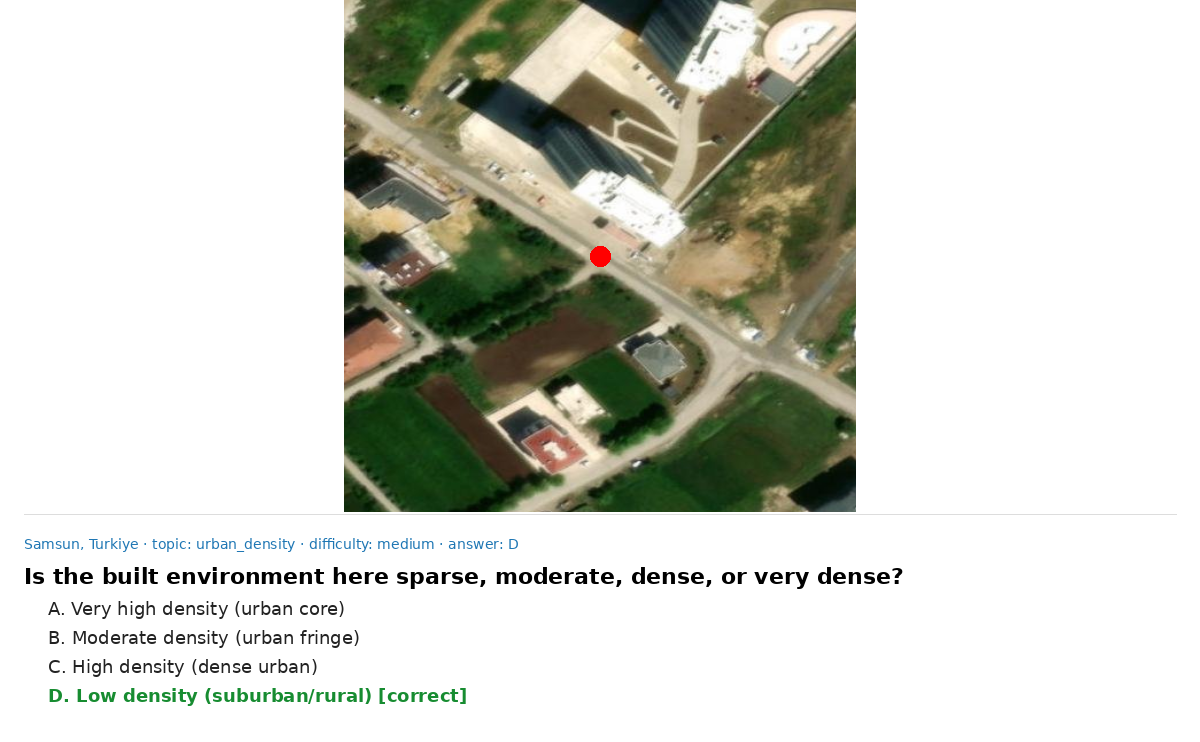
\includegraphics[width=0.9\linewidth]{examples/ex_urban_density.png}
  \caption{\texttt{urban\_density} --- building density category.}
\end{figure}

\begin{figure}[H]
  \centering
  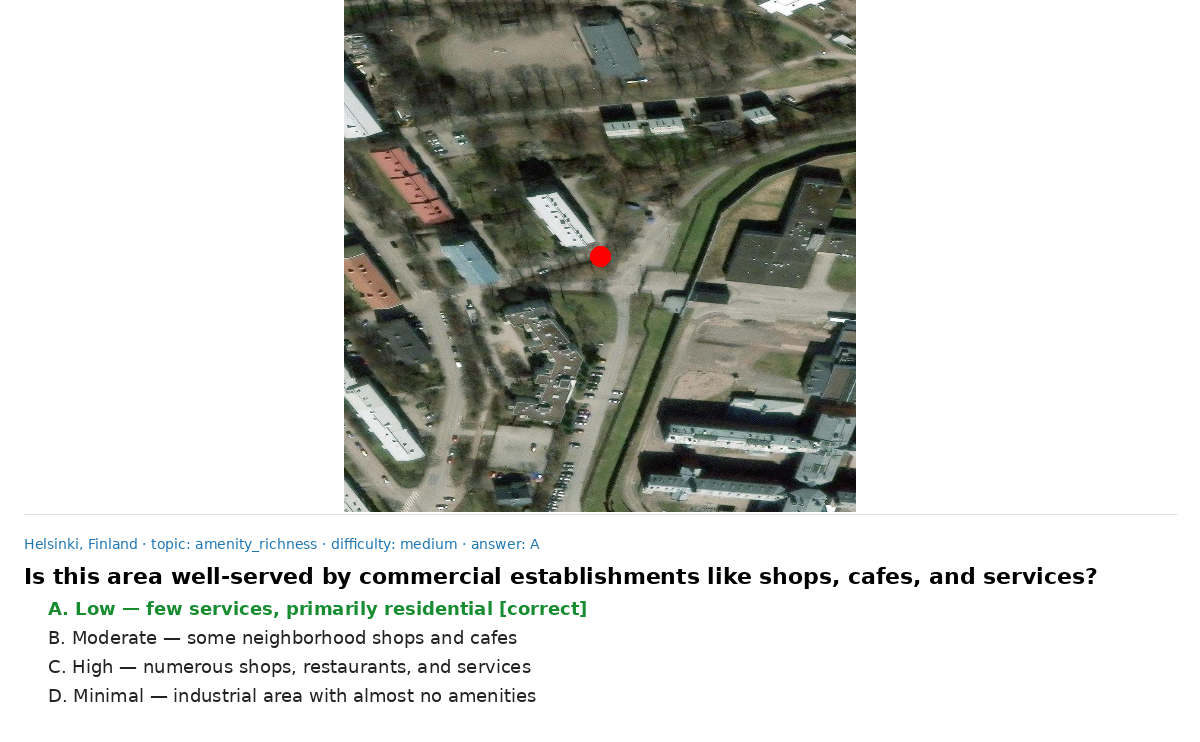
\includegraphics[width=0.9\linewidth]{examples/ex_amenity_richness.png}
  \caption{\texttt{amenity\_richness} --- shops, cafés, services density.}
\end{figure}

\begin{figure}[H]
  \centering
  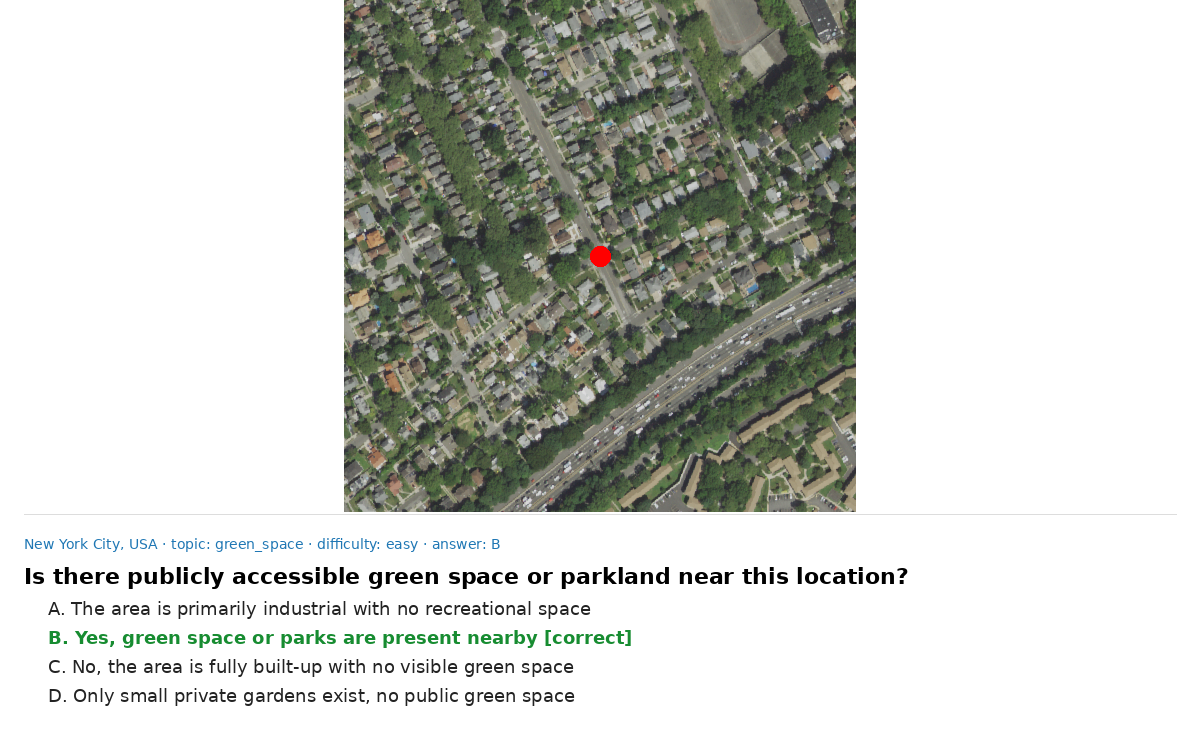
\includegraphics[width=0.9\linewidth]{examples/ex_green_space.png}
  \caption{\texttt{green\_space} --- vegetation presence and proximity.}
\end{figure}

\begin{figure}[H]
  \centering
  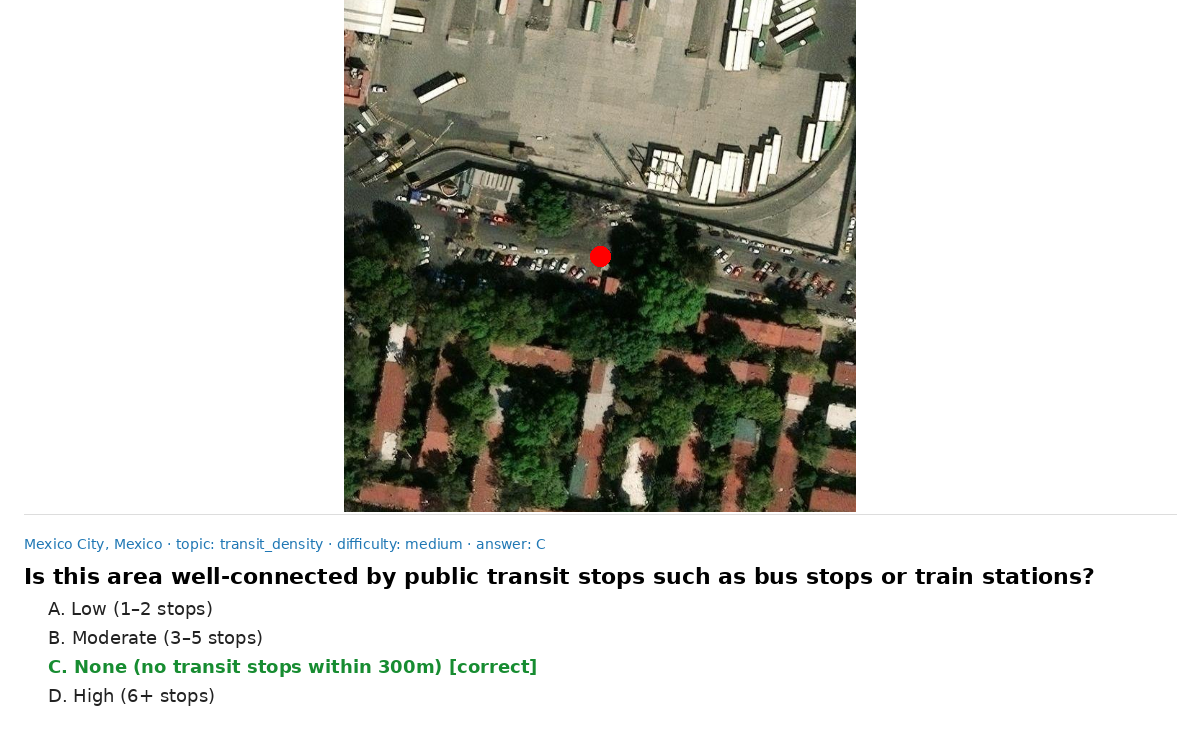
\includegraphics[width=0.9\linewidth]{examples/ex_transit_density.png}
  \caption{\texttt{transit\_density} --- transit stops within 300\,m.}
\end{figure}

\begin{figure}[H]
  \centering
  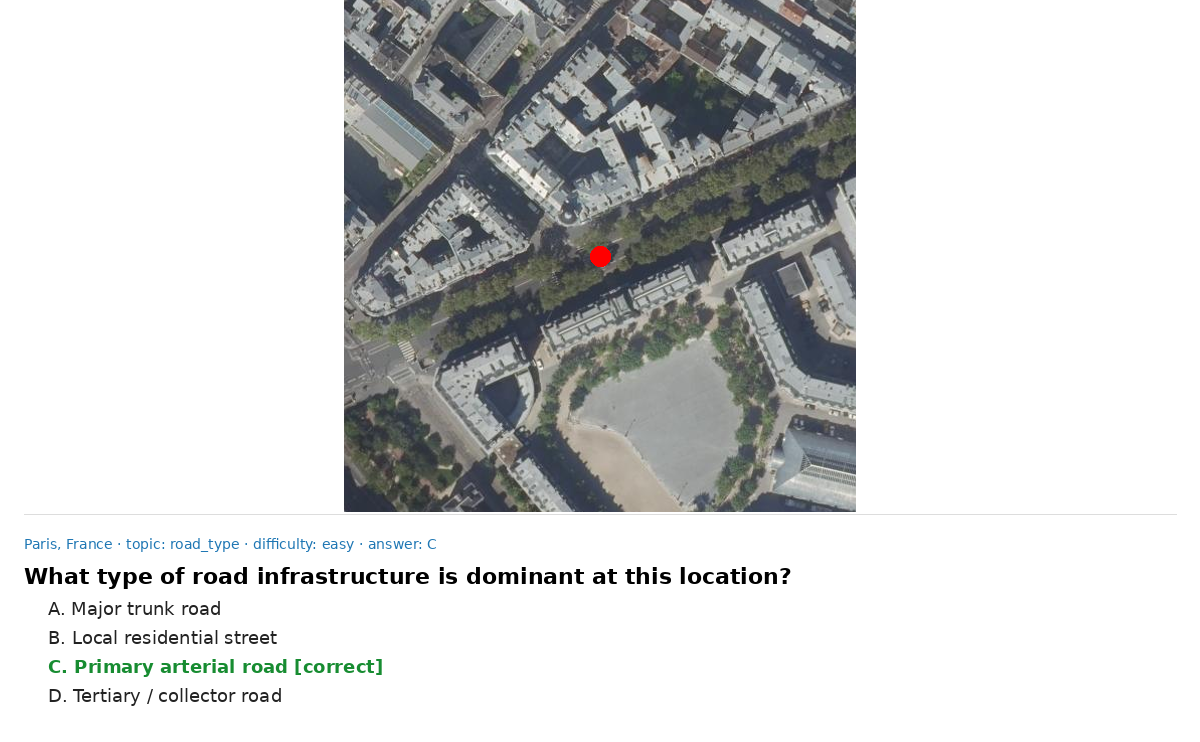
\includegraphics[width=0.9\linewidth]{examples/ex_road_type.png}
  \caption{\texttt{road\_type} --- OSM road category.}
\end{figure}

\begin{figure}[H]
  \centering
  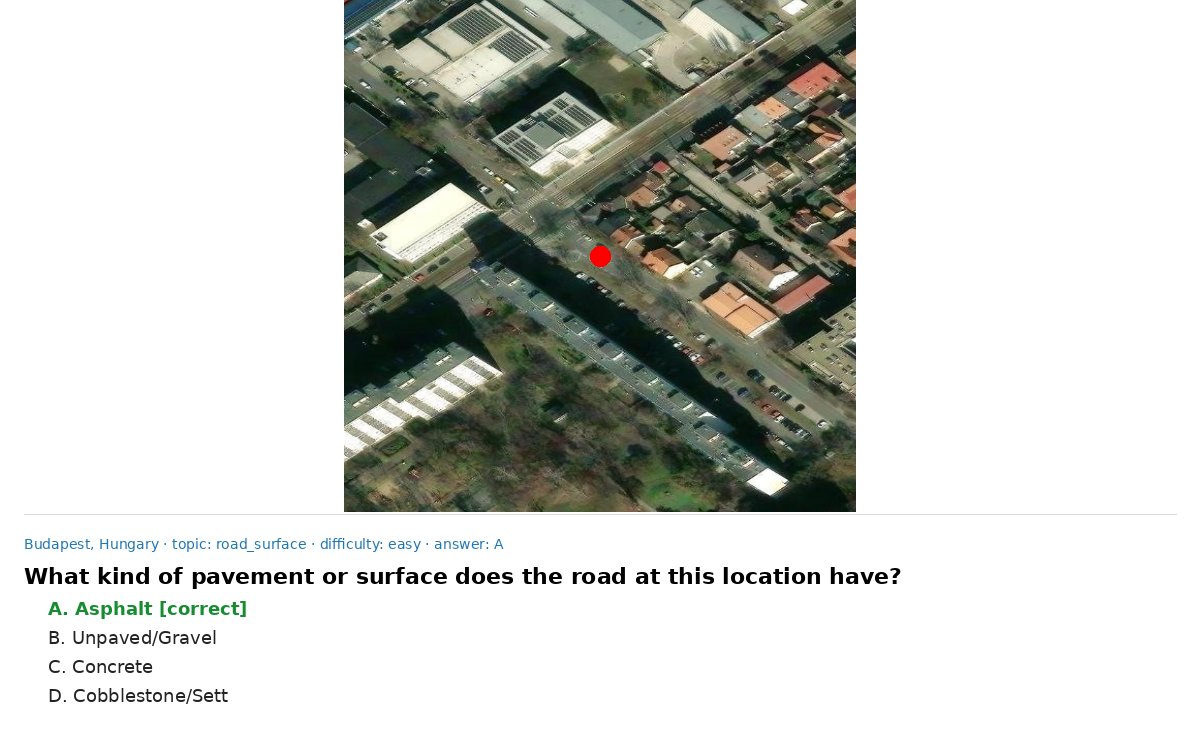
\includegraphics[width=0.9\linewidth]{examples/ex_road_surface.png}
  \caption{\texttt{road\_surface} --- asphalt, cobblestone, unpaved, concrete.}
\end{figure}

\begin{figure}[H]
  \centering
  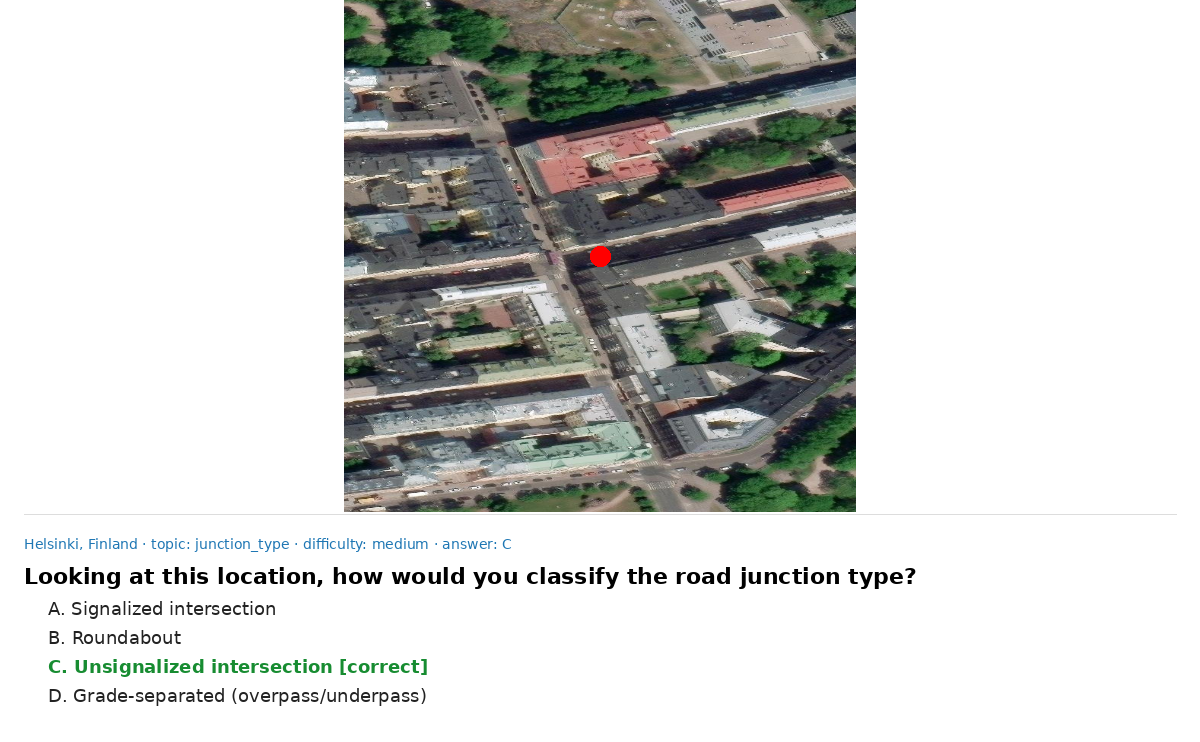
\includegraphics[width=0.9\linewidth]{examples/ex_junction_type.png}
  \caption{\texttt{junction\_type} --- intersection topology.}
\end{figure}

\subsection{Cross-view geolocalisation examples}

\begin{figure}[H]
  \centering
  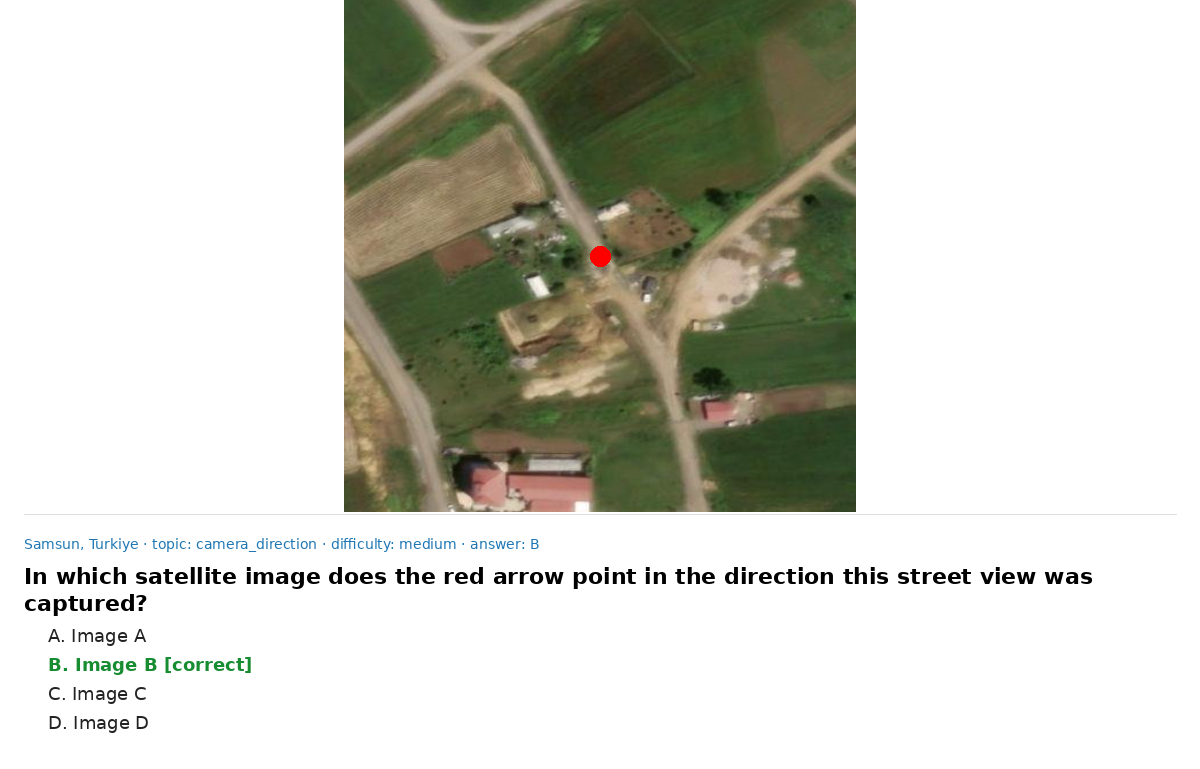
\includegraphics[width=0.95\linewidth]{examples/ex_camera_direction.png}
  \caption{\texttt{camera\_direction} --- the satellite shows four
  arrows (one per option); a single Street View image is shown
  alongside; the model must identify which compass direction the
  photo was taken from.}
\end{figure}

\begin{figure}[H]
  \centering
  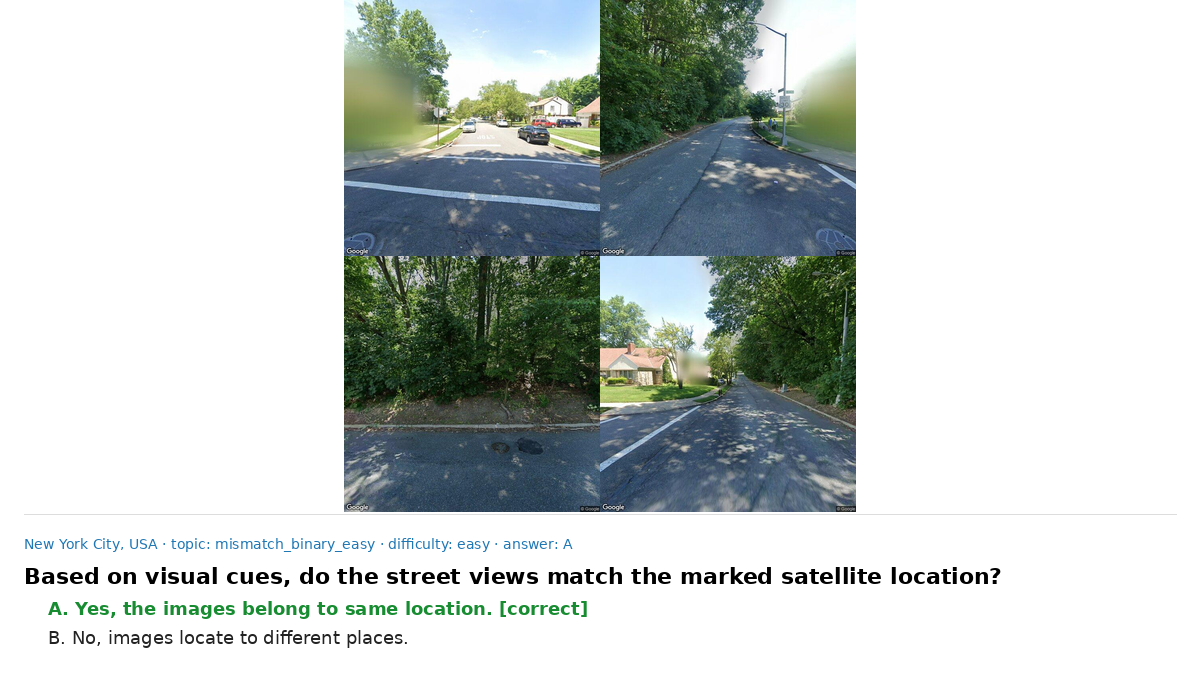
\includegraphics[width=0.9\linewidth]{examples/ex_mismatch_binary_easy.png}
  \caption{\texttt{mismatch\_binary\_easy} --- does this 4-angle
  Street View grid belong to the satellite tile shown? Distractor
  drawn from a different city.}
\end{figure}

\begin{figure}[H]
  \centering
  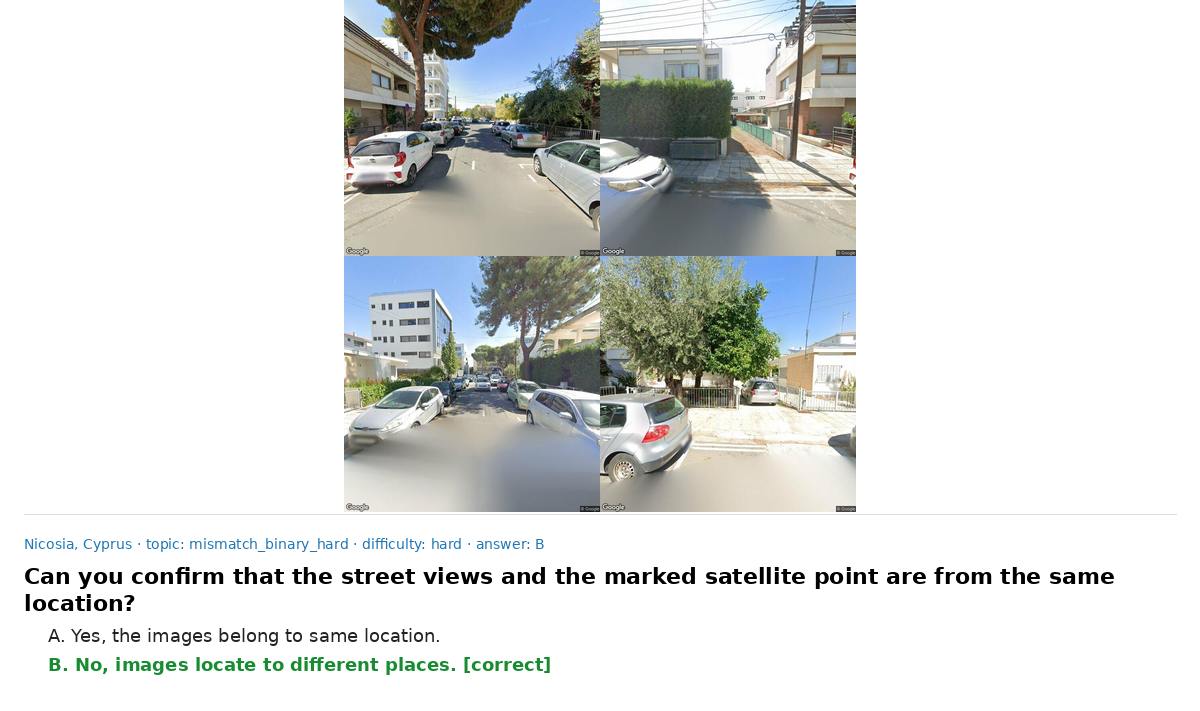
\includegraphics[width=0.9\linewidth]{examples/ex_mismatch_binary_hard.png}
  \caption{\texttt{mismatch\_binary\_hard} --- same task as above
  but the distractor is sampled from the \emph{same} city, removing
  vegetation- and signage-based shortcuts.}
\end{figure}

\begin{figure}[H]
  \centering
  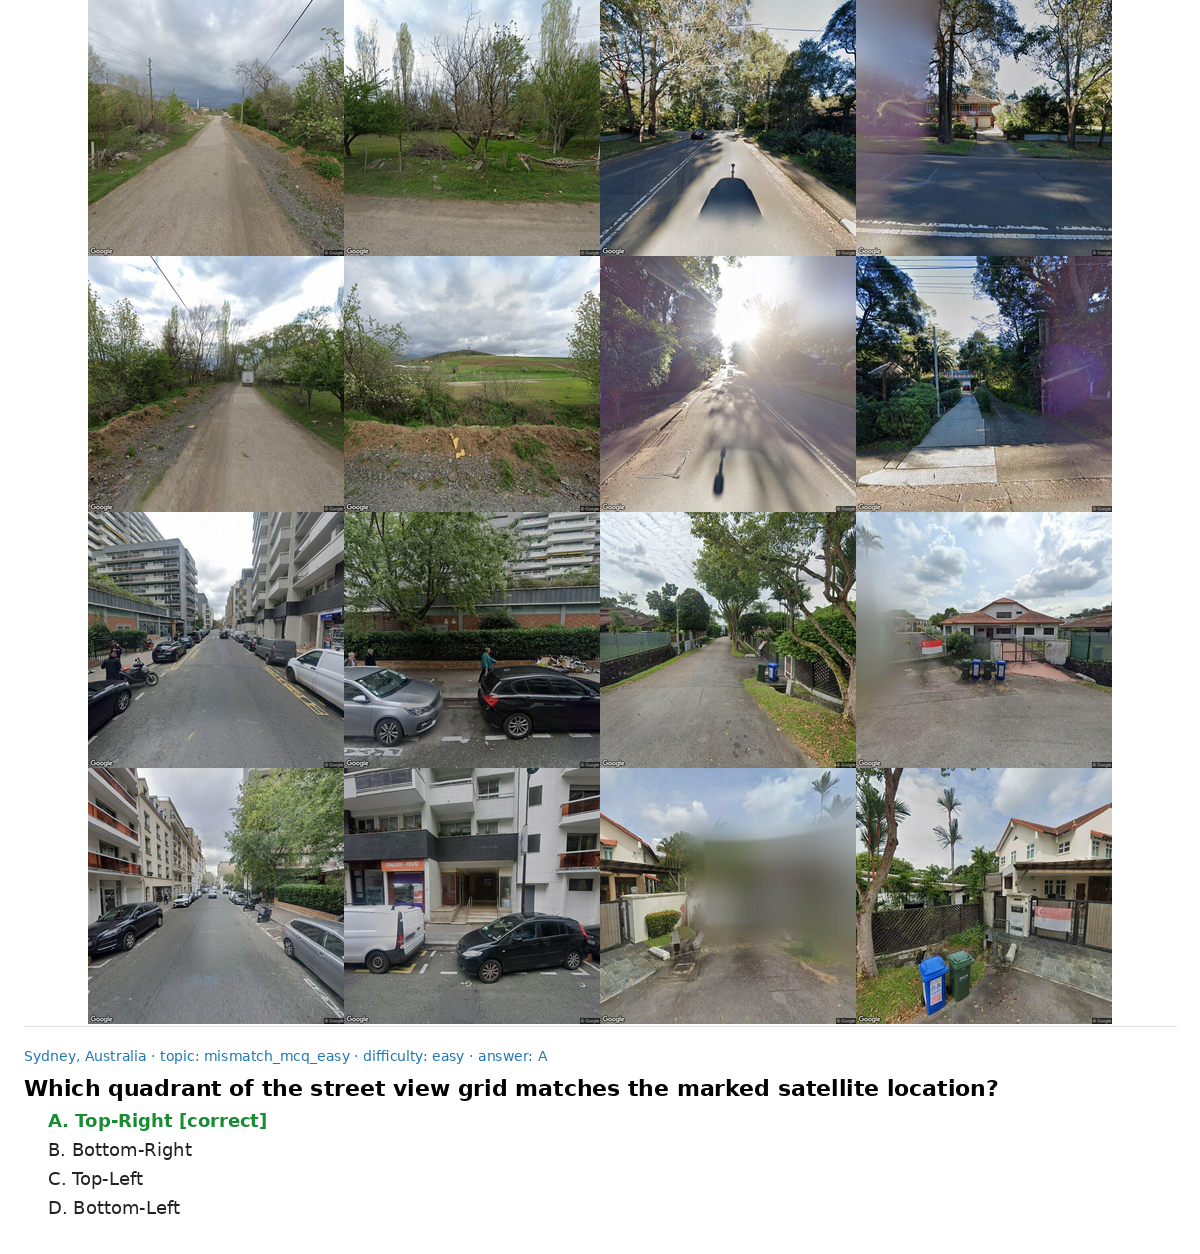
\includegraphics[width=\linewidth]{examples/ex_mismatch_mcq_easy.png}
  \caption{\texttt{mismatch\_mcq\_easy} --- pick which of four
  4-angle Street View composites matches the satellite (cross-city
  distractors).}
\end{figure}

\begin{figure}[H]
  \centering
  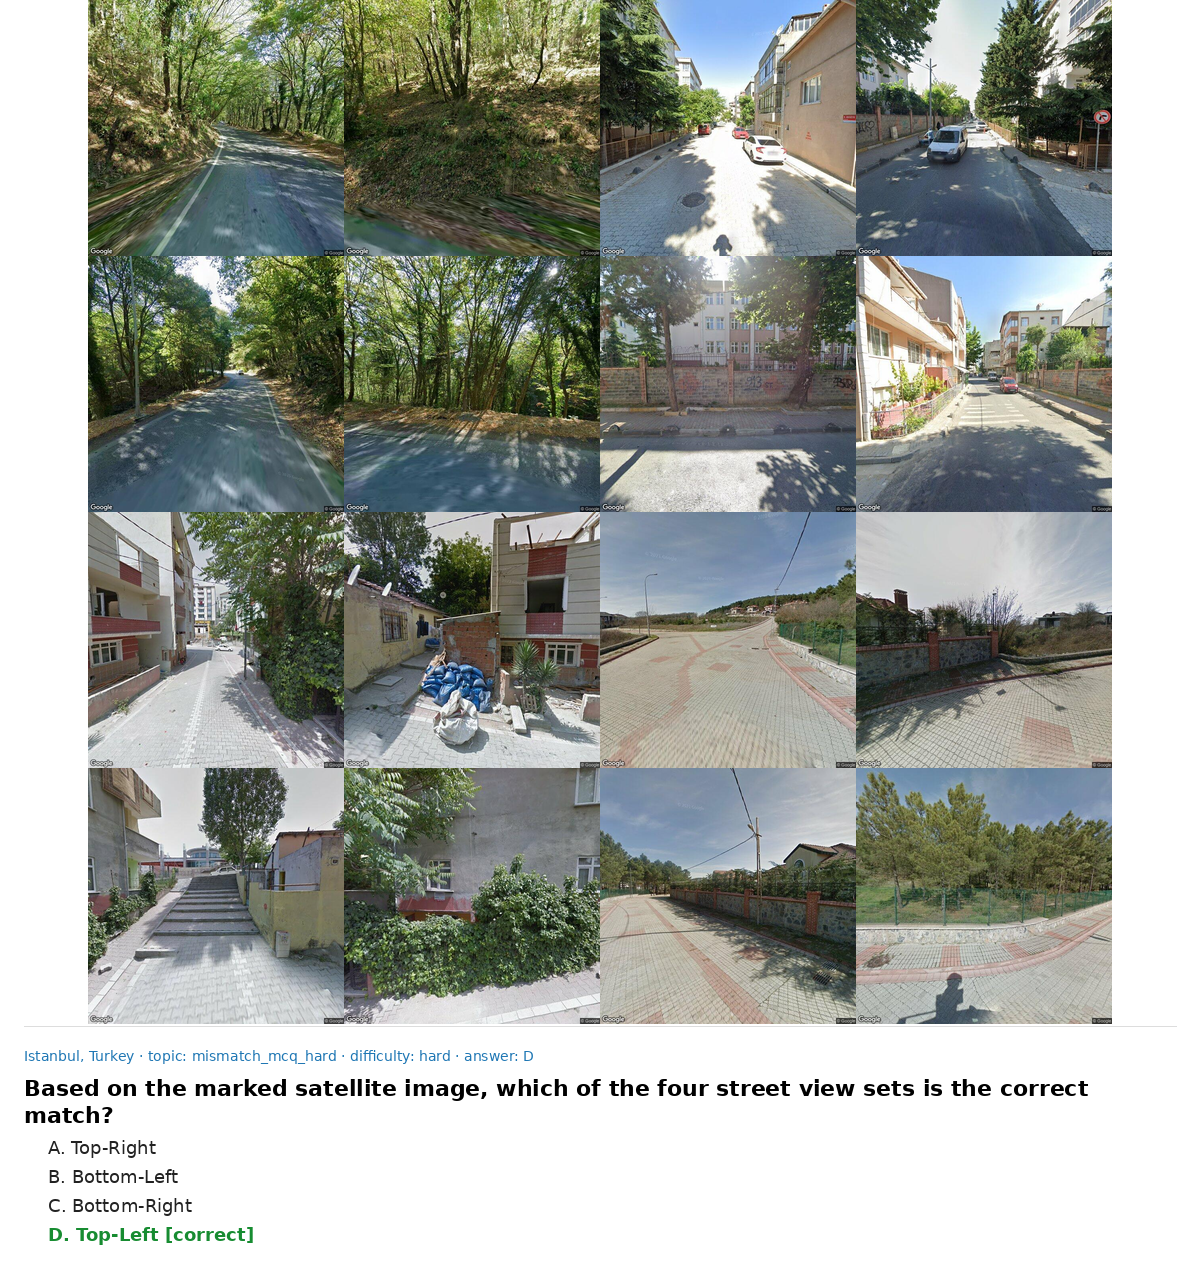
\includegraphics[width=\linewidth]{examples/ex_mismatch_mcq_hard.png}
  \caption{\texttt{mismatch\_mcq\_hard} --- same task as above but
  all four candidates are drawn from the same city as the target.
  This is the hardest task in the corpus.}
\end{figure}

% =====================================================================
\section{Split Strategies in Detail}
% =====================================================================

\paragraph{splits\_per\_city.}
Within each city, locations are randomly assigned to train (80\%)
or validation. The model sees \emph{every} city during training;
validation tests whether the model can generalise to new locations
within familiar urban contexts.

\paragraph{splits\_seen\_unseen.}
Cities are partitioned into 32 \emph{seen} cities (all training
locations) and 8 \emph{unseen} cities (all validation locations).
The model never observes a single location from a held-out city.
The 8 unseen cities are:
Cape Town, Chicago, Istanbul, Moscow, Rio de Janeiro, Seoul,
Singapore, Sydney.

\paragraph{benchmark.}
A held-out 5{,}240-record evaluation set drawn from a disjoint mix
of seen and unseen cities (\texttt{benchmark\_city\_type =
seen\_city / unseen\_city}). Shipped as two parallel files;
\texttt{benchmark\_public.jsonl} sets \texttt{"answer": null}, and
\texttt{benchmark\_with\_answers.jsonl} contains the gold labels.

\begin{figure}[H]
  \centering
  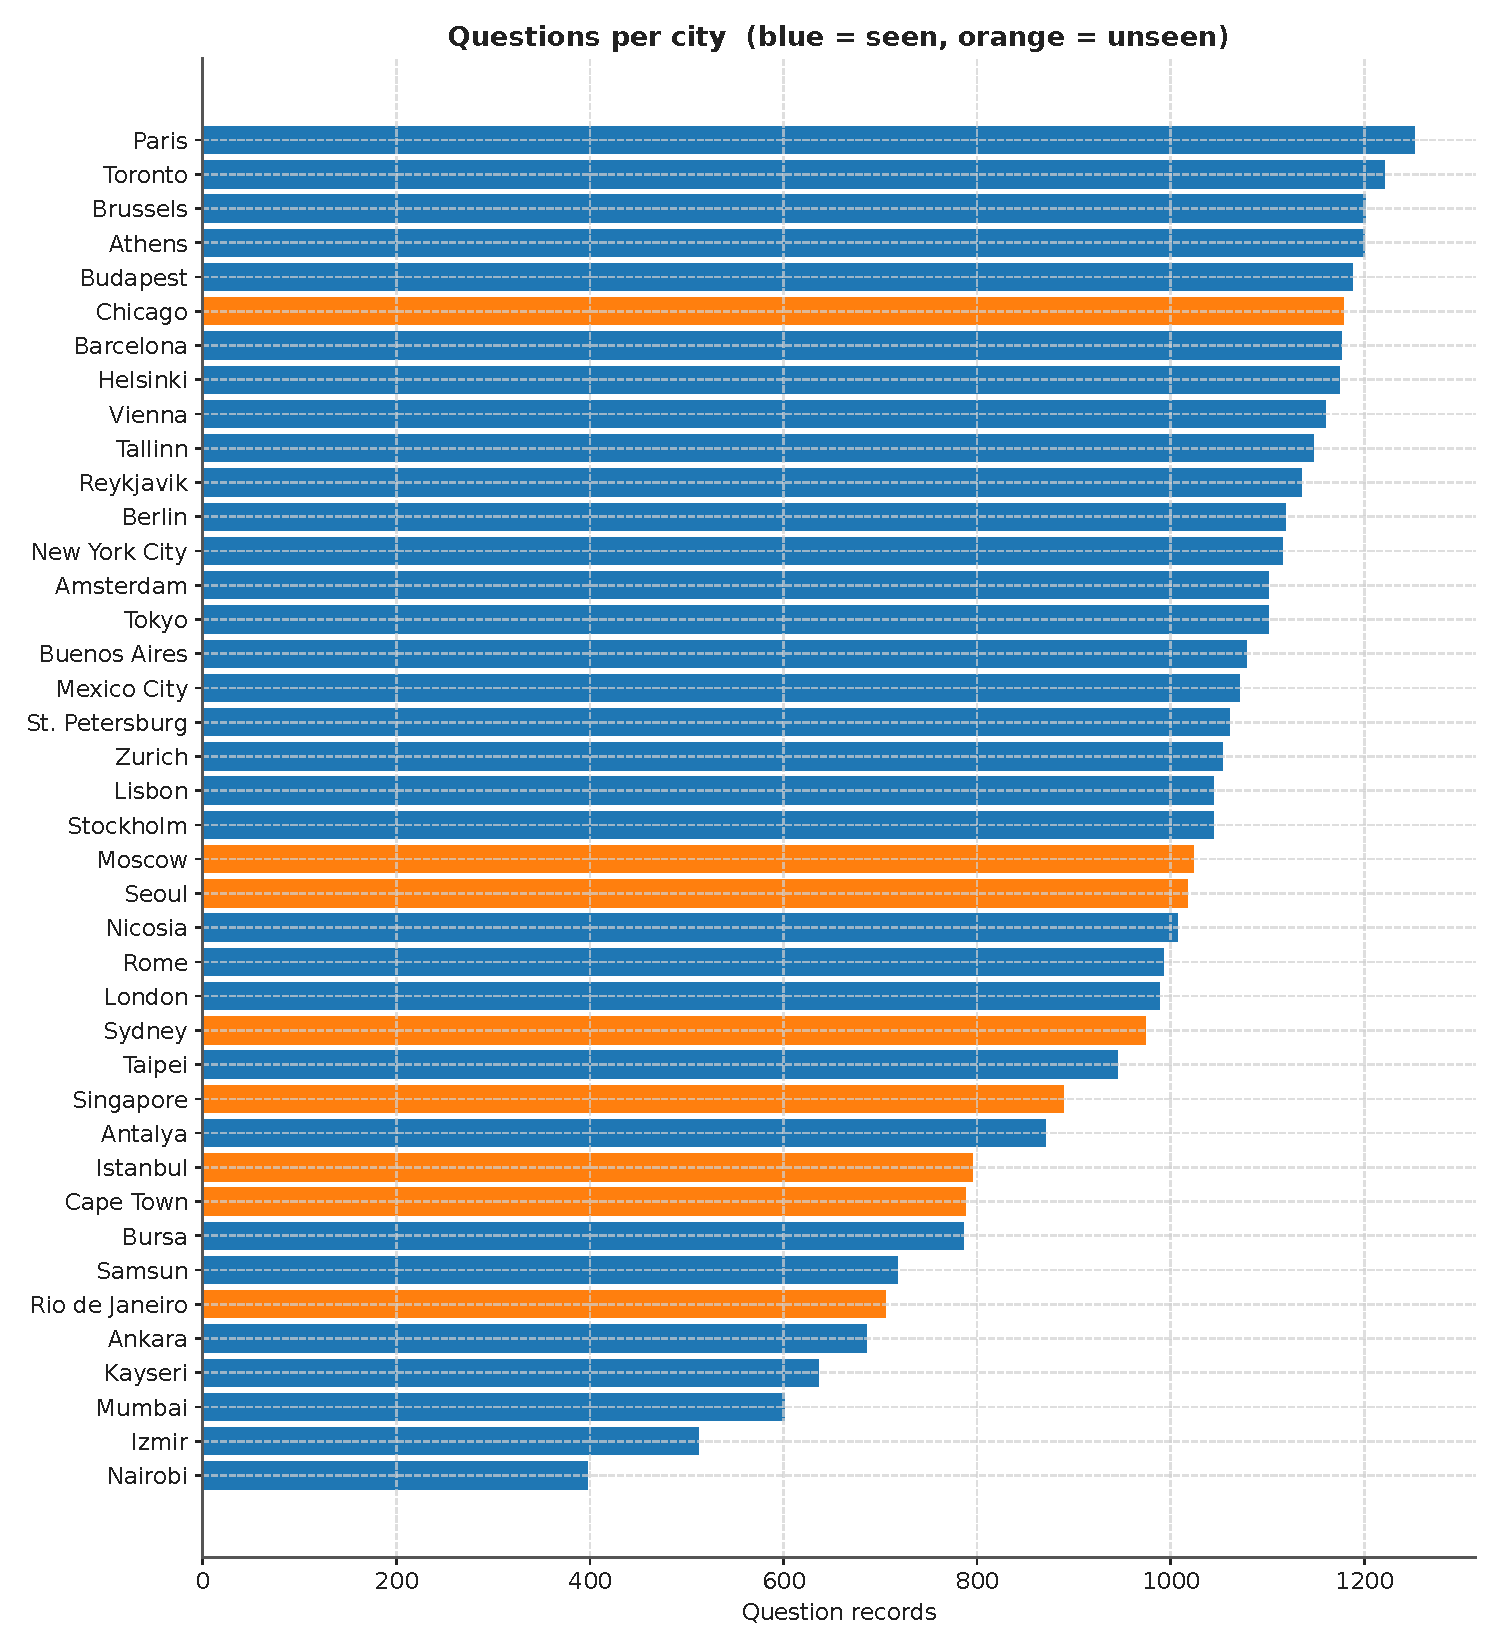
\includegraphics[width=0.92\linewidth]{figures/fig02_cities.pdf}
  \caption{Question records per city across all released splits.
  Blue = seen city, orange = unseen city.}
  \label{fig:cityrecords}
\end{figure}

% =====================================================================
\section{File Layout and JSONL Schema}
% =====================================================================

The released archive is laid out as:

\begin{lstlisting}
EODATA_compressed_final/
|-- README.md
|-- composite_utils.py            <- only file the dataloader needs
|-- benchmark/
|   |-- benchmark_public.jsonl
|   |-- benchmark_with_answers.jsonl
|   `-- images/{sat,sv}/
|-- splits_per_city/
|   |-- train.jsonl
|   |-- validation.jsonl
|   `-- images/{sat,sv}/
`-- splits_seen_unseen/
    |-- train.jsonl
    |-- validation.jsonl
    `-- images/{sat,sv}/
\end{lstlisting}

\subsection{Per-record JSONL fields}

\renewcommand{\arraystretch}{1.15}
\begin{tabularx}{\linewidth}{@{}>{\ttfamily\small}l>{\itshape\small}l X@{}}
\toprule
\textnormal{\textbf{Field}}      & \textbf{Type}   & \textbf{Description} \\
\midrule
question\_id      & string  & Unique per (sample, topic, variant). \\
sample\_id        & string  & Location ID, e.g.\ \texttt{amsterdam\_0017}. \\
city, country     & string  & Place metadata. \\
latitude, longitude & float & WGS-84 of the sample point. \\
land\_use         & string  & OSM-derived dominant land use. \\
streetview\_count & int     & Number of SV angles available (usually 4). \\
question          & string  & MCQ question text. \\
options           & dict    & \texttt{\{A,B,C,D\} -> text}. \\
answer            & string  & Letter; \texttt{null} in benchmark\_public. \\
topic             & string  & One of the 14 topics. \\
difficulty        & string  & \texttt{easy} / \texttt{medium} / \texttt{hard}. \\
image\_mode       & string  & Which visual to assemble (see below). \\
images            & dict    & Paths + provenance for the raw images. \\
split             & string  & \texttt{train} / \texttt{validation} / \texttt{benchmark}. \\
city\_type        & string  & \texttt{seen} / \texttt{unseen} (seen\_unseen only). \\
benchmark\_city\_type & string & \texttt{seen\_city} / \texttt{unseen\_city}. \\
\midrule
\multicolumn{3}{l}{\textit{Topic-specific fields:}} \\
query\_stv\_path, query\_stv\_angle  & string & The single SV shown for \texttt{camera\_direction}. \\
option\_arrow\_angles                & dict   & MCQ-option $\rightarrow$ angle \emph{name} (\texttt{along\_fwd}, \texttt{cross\_left}, etc.); \texttt{composite\_utils.py} converts to bearings. \\
option\_stv\_paths                   & dict   & MCQ-option $\rightarrow$ list of 4 SV paths (\texttt{mismatch\_mcq}). \\
mismatch\_strategy                   & string & \texttt{same\_city} / \texttt{cross\_city}. \\
mismatch\_is\_match                  & bool   & Binary mismatch ground truth. \\
mismatch\_negative\_stv\_paths       & list   & 4 SV paths of the non-matching location (all \texttt{mismatch\_binary} non-match records, both easy and hard). \\
generation\_method                  & string & Always \texttt{template} in the current release. \\
\bottomrule
\end{tabularx}

\subsection{image\_mode dispatch}

\begin{tabularx}{\linewidth}{@{}>{\ttfamily\small}l X@{}}
\toprule
\textnormal{\textbf{image\_mode}} & \textbf{Visual rendered for the model} \\
\midrule
satellite\_marked     & Raw satellite with a red dot at the sample centre. \\
satellite\_arrow      & Raw satellite with a labelled arrow per MCQ option. \\
streetview\_composite & 2$\times$2 grid of the four SV angles of the query sample. \\
streetview\_binary    & 2$\times$2 grid of the \emph{non-matching} sample (both \texttt{mismatch\_binary\_easy} and \texttt{mismatch\_binary\_hard} non-match records). \\
streetview\_mega      & 4$\times$4 mega-grid: four candidate locations,
                        four angles each, for \texttt{mismatch\_mcq}. \\
\bottomrule
\end{tabularx}

\noindent\textit{Note.} \texttt{composite\_utils.py} also implements
\texttt{satellite\_only} and \texttt{streetview\_single} dispatch
branches; neither is assigned as an \texttt{image\_mode} value in the
released JSONL files (they are reserved for fallback / inline-query
uses).

\subsection{Dataloader excerpt}

\begin{lstlisting}[language=Python]
import json
from composite_utils import get_images_for_question

base = "/path/to/EODATA_compressed_final/splits_per_city"
with open(f"{base}/train.jsonl") as f:
    record = json.loads(f.readline())

info = get_images_for_question(record, base_dir=base)
primary = info["primary"]                # PIL.Image
options = info.get("options", {})        # dict for MCQ tasks
query   = info.get("query_sv")           # PIL.Image for camera_direction
\end{lstlisting}

\noindent The single file \texttt{composite\_utils.py} re-assembles every
visual on demand --- the dataset ships only raw satellite PNGs and
raw SV JPEGs ($\sim$7\,GB total). The full pre-rendered edition
(\texttt{EODATA\_final}, $\sim$221\,GB) is functionally identical but
trades disk for runtime.

% =====================================================================
\section{Limitations \& Known Issues}
\label{sec:limits}
% =====================================================================

\begin{itemize}[itemsep=3pt]
  \item \textbf{Correct-letter imbalance.} Within the 39{,}155-record
        release, answers A and B each occur $\sim$11{,}300 times while
        C and D each occur $\sim$8{,}300 times (Fig.~\ref{fig:diffans}).
        This is a known artefact of the option-shuffling RNG: the
        per-question seed (\texttt{sample\_id} + topic) is not
        uniformly distributed over the 4! permutations. Always-A
        scores $\sim$29\% accuracy.
  \item \textbf{Country-label duplication.} The raw JSONL contains
        both \texttt{Turkey} and \texttt{Turkiye} as separate strings;
        treating them as the same country reduces the unique-country
        count from 33 to \textbf{32}. All statistics in this report
        use the normalised count.
  \item \textbf{Sparse \texttt{building:levels} in some cities.}
        São Paulo and Singapore have sparse height tags in OSM,
        which depresses \texttt{building\_height} records for those
        cities. (São Paulo is not in the final release; Singapore is
        held-out as an unseen city.)
  \item \textbf{Street View coverage holes.} Canary Wharf
        (London) has no outdoor SV; affected locations were dropped
        at Step 03.
  \item \textbf{Overpass reliability.} For large bounding boxes
        (e.g.\ historical São Paulo runs), the OSM Overpass API
        sometimes timed out; the pipeline retries with backoff and
        skips samples without context tags.
  \item \textbf{Satellite-tile rejection.} Tiles smaller than
        5\,kB are auto-rejected and the next provider is tried;
        in the final release this fallback was not triggered.
  \item \textbf{Difficulty labels.} The \texttt{difficulty} field
        is a template-level annotation, not a model-difficulty
        estimate. The "hard" bucket is dominated by
        \texttt{mismatch\_*\_hard} questions (Fig.~\ref{fig:topicdiff}).
  \item \textbf{\texttt{water\_proximity} is defined but unreleased.}
        \texttt{src/config.py} lists \texttt{water\_proximity} in
        \texttt{ENABLED\_QUESTION\_TYPES}, but no records of this
        topic survive the validation step in the final release. All
        statistics in this report use the 14 topics actually present
        in the JSONL.
\end{itemize}

% =====================================================================
\section{Reproducibility}
% =====================================================================

The pipeline depends on:
\begin{itemize}[itemsep=0pt]
  \item OpenStreetMap snapshot at run time (Overpass API).
  \item Google Earth Engine for satellite tiles (NAIP, IGN, S2 fallback).
  \item Google Street View Static API for SV imagery.
  \item ESRI World Imagery REST endpoint for default global satellite.
\end{itemize}

\noindent Option ordering is deterministic given a fixed OSM snapshot,
since the per-question RNG seed combines \texttt{sample\_id} and
\texttt{topic}. The released JSONL is therefore a bit-exact snapshot
of one pipeline run; re-running on a new OSM snapshot may shift
small numbers of OSM-tag-dependent answers (e.g.\ a newly tagged park
flipping a \texttt{green\_space} answer).

\begin{infobox}[Required to consume the dataset]
Pillow $\geq$ 10.0 (only dependency of \texttt{composite\_utils.py}).\\
PyTorch is required only if you use the example dataloader.
\end{infobox}

% =====================================================================
\section{Summary}
% =====================================================================

EOLLM is a deterministic, multi-modal VQA corpus that pairs satellite
and Street View imagery across 40 cities and asks 14 task families
covering urban understanding and cross-view geolocalisation. The
release contains \textbf{39{,}155 question records} over \textbf{4{,}168
unique locations}, packaged at $\sim$7\,GB with three split strategies
that target both in-distribution and geographic-generalisation
evaluation. All ground truth is OSM-derived; option shuffling is
reproducible by construction; the dataloader is a single-file Pillow
script. The dataset is intended as a benchmark for Vision-Language
Models that must reason jointly about overhead and ground-level views
of the same place.

\end{document}
